% ------------------------------------------------------------------------
% ------------------------------------------------------------------------
% Modelo de Trabalho Acadêmico utilizando repUERJ 
% tese de doutorado, dissertação de mestrado e trabalhos monográficos em geral
%
% * Este aquivo está editado na codificação de caracteres UTF-8.
%
% ------------------------------------------------------------------------
% ------------------------------------------------------------------------
%
\documentclass[a4paper,12pt,oneside,onecolumn,final,fleqn]{repUERJ}

% ---
% Pacotes fundamentais 
% ---
\usepackage[brazil]{babel}  % adequacao para o portugues Brasil
\usepackage[utf8]{inputenc} % Determina a codificacao utiizada
                            % (conversão automática dos acentos)
\usepackage{makeidx}        % Cria o indice
\usepackage{hyperref}       % Controla a formacao do indice
\usepackage{lastpage}       % Usado pela Ficha catalografica
\usepackage{indentfirst}    % Indenta o primeiro paragrafo de cada secao.
\usepackage{xcolor}          % Controle das cores
\usepackage{graphicx}       % Inclusao de graficos
\usepackage{subfig}
\usepackage{amsmath}        % pacote matemático
\usepackage{amssymb}
\usepackage{amsthm}
\usepackage{multirow}
\usepackage{hhline}
\usepackage{tikz}
\usetikzlibrary{calc}

\usepackage{setspace}
\usepackage{caption}
\captionsetup[table]{singlelinecheck=false}
\captionsetup[figure]{slc=off}
\captionsetup{font=singlespacing}
\captionsetup{tableposition=top}

\theoremstyle{plain}
\newtheorem{thm}{Theorem}[chapter] % reset theorem numbering for each chapter

\theoremstyle{definition}
\newtheorem{defn}[thm]{Definition} % definition numbers are dependent on theorem numbers
\newtheorem{exmp}[thm]{Example}

\usepackage{macrosfabbri-basic}
\usepackage{macrosfabbri-dg}
\newcommand{\RNum}[1]{\uppercase\expandafter{\romannumeral #1\relax}}
\newcommand{\rnum}[1]{\expandafter{\romannumeral #1\relax}}
\renewcommand{\myparagraph}{\noindent\textbf}

% ---
% Pacote auxiliar para as normas da UERJ
% ---
\usepackage[frame=no,algline=yes,font=default]{repUERJformat}
% ---
% Pacotes de citacoes
% ---
\usepackage[alf]{abntex2cite}

% *****************************************************************************
% *****************************************************************************
% Comandos especificos deste exemplo 
% * podem ser retirados na edicao de um novo documento
% *****************************************************************************
% *****************************************************************************

\newcommand{\comando}[1]{\texttt{\bs #1}}
\newcommand{\opcoes}[1]{\texttt{[}\textsl{#1}\texttt{]}}
\newcommand{\param}[1]{\texttt{\{}\textsl{#1}\texttt{\}}}
\newcommand{\BibTeX}{{{Bib}}\TeX}
\newcommand{\repUERJ}{\textsf{repUERJ}}
\newcommand{\formato}[1]{\begin{flushleft}{#1}\end{flushleft}}
\newcommand{\bs}{\textbackslash}
\def\ReduceAfterCaptionfigspace{}

% *****************************************************************************
% *****************************************************************************
% Informacoes de autoria e institucionais
% *****************************************************************************
% *****************************************************************************

%-----------------------------------------------------------------------
% Imagens pretextuais (precisam estar no mesmo diretorio deste arquivo .tex)
%-----------------------------------------------------------------------

\logo{logo_uerj_cinza.png}

%-----------------------------------------------------------------------
% Informacoes da instituicao
%-----------------------------------------------------------------------

\instituicao{Universidade do Estado do Rio de Janeiro}
            {Instituto Politécnico} 
            {Departamento de Modelagem Computacional}  
            {}

%-----------------------------------------------------------------------
% Informacoes da autoria do documento
%-----------------------------------------------------------------------

\autor{Pedro Felipe Pena}{Barata}

\titulo{Técnicas de reconstrução 3D - ????}
\palavraschaves{Reconstrução densa}{Nuvem de pontos}{SfM}{???}

%\title{Treinamento de um novo rastreador de bordas para múltiplos vídeos de ondas oceânicas}
%\keywords{Contour Detection}{Edge Fragments}{Machine Learning}{Water Waves}

\orientador{Prof.\ Dr.} 
           {Ricardo}{Fabbri} 
           {Instituto Politécnico -- UERJ}

%-----------------------------------------------------------------------
% Titulacao (Doutor, Mestre, Bacharel, Licenciado) e Curso
%-----------------------------------------------------------------------

\grau{Graduado}  
\curso{Engenharia de Computação} 
\areadeconcentracao{}

%-----------------------------------------------------------------------
% Informacoes adicionais (local, data e paginas)
%-----------------------------------------------------------------------

\local{Nova Friburgo} 
\data{02}{09}{2017} 

% *****************************************************************************
% *****************************************************************************
% Configurações de aparência do PDF final
% *****************************************************************************
% *****************************************************************************

% alterando o aspecto da cor azul
\definecolor{blue}{RGB}{41,5,195}
\definecolor{apricot}{RGB}{251,206,177}

% informações do PDF
\hypersetup{
  %backref=true,
  %pagebackref=true,
  %bookmarks=true,                  % show bookmarks bar?
  unicode=false,
  pdftitle={\UERJtitulo},
  pdfauthor={\UERJautor},
  pdfsubject={\UERJpreambulo},
  pdfkeywords={PALAVRAS}{CHAVES}{\chaveA}{\chaveB}{\chaveC}{\chaveD},
  pdfproducer={\packagename}, % producer of the document
  pdfcreator={\UERJautor},
  colorlinks=true,                  % false: boxed links; true: colored links
  linkcolor=blue,                   % color of internal links blue
  citecolor=red,                    % color of links to bibliography blue
  filecolor=magenta,                % color of file links magenta
  urlcolor=green,
  bookmarksdepth=4
}

% *****************************************************************************
% *****************************************************************************
% Início do documento
% *****************************************************************************
% *****************************************************************************

% ---
% compila o indice
% ---
\makeindex
% ---

% *****************************************************************************
% *****************************************************************************

\begin{document}
\pagestyle{empty}
\begin{tikzpicture}[overlay,remember picture]
    \draw [line width=2pt ]
        ($ (current page.north west) + (2cm,-2cm) $)
        rectangle
        ($ (current page.south east) + (-1cm,1.5cm) $);
    \draw [line width=1pt]
        ($ (current page.north west) + (2.1cm,-2.1cm) $)
        rectangle
        ($ (current page.south east) + (-1.1cm,1.6cm) $);
\end{tikzpicture}
% ----------------------------------------------------------
% ELEMENTOS PRE-TEXTUAIS
% ----------------------------------------------------------

\frontmatter

% ----------------------------------------------------------
% Capa e a folha de rosto
% ----------------------------------------------------------

\capa
\pagestyle{empty}
\begin{tikzpicture}[overlay,remember picture]
    \draw [line width=2pt ]
        ($ (current page.north west) + (2cm,-2cm) $)
        rectangle
        ($ (current page.south east) + (-1cm,1.5cm) $);
    \draw [line width=1pt]
        ($ (current page.north west) + (2.1cm,-2.1cm) $)
        rectangle
        ($ (current page.south east) + (-1.1cm,1.6cm) $);
\end{tikzpicture}
\folhaderosto* % modelo de folha de rosto para monografia do Inst. Fís. UERJ

% ----------------------------------------------------------
% Inserir a ficha catalografica
% ----------------------------------------------------------

%\fichacatalografica{fichacatalografica.pdf}

% ----------------------------------------------------------
% Folha de aprovacao
% ----------------------------------------------------------

\begin{folhadeaprovacao}
  \assinatura{Banca1\par
  \UERJorientadorinstituicao}
  \assinatura{Banca2\par
  \UERJorientadorinstituicao}

\end{folhadeaprovacao}

% ----------------------------------------------------------
% Dedicatoria
% ----------------------------------------------------------

%\pretextualchapter{Dedicatória}

%\vfill

% ----------------------------------------------------------
% Agradecimentos
% ----------------------------------------------------------

\pretextualchapter{Agradecimentos}
%
%À Deus pela minha vida.
%
%À minha família por ser minha fortaleza e meu porto.
%
%À Anna Cruz por tudo.
%
%Ao meu orientador pela dedicação.

% ----------------------------------------------------------
% Epigrafe
% ----------------------------------------------------------

\pretextualchapter{}

%  \vfill\
%  \begin{flushright}
%    God grant me the serenity to accept the things I cannot change,\\
%    Courage to change the things I can change,\\
%     And wisdom to know the difference.\\
%    \textsl{Reinhold Niebuhr}
%  \end{flushright}

% ----------------------------------------------------------
% RESUMO
% ----------------------------------------------------------

\pretextualchapter{Resumo}

\referencia

%Os vídeos de ondas de água são desafiadores para rastrear e reconstruir devido a alta transparência, 
%especularidades, baixo contraste e padrões repetitivos, especialmente no
%cenário de tanques de água. A maioria das abordagens não são especificamente 
%projetadas para imagens de água, ou são específicas de uma forma que não 
%generaliza para vários tipos de imagens. Criamos um detector de borda de subpíxel 
%e um \textit{linker} especificamente para vídeos de água, 
%aprendendo geometria e topologia em um conjunto de treinamento, para uso em sistemas recentes de 
%fotogrametria com base em curva 3D. A abordagem, no entanto, generaliza à criação de 
%detectores de \emph{features} geométricas específicas para uma série de aplicações adicionais.
%No cenário geral -- sem textura abundante, 
%curvas e superfícies seguindo modelos específicos ou limitando a complexidade da
%cena -- a 
%reconstrução 3D geralmente produz nuvens pontuais não organizadas, malhas ou representações de voxel, 
%com algumas técnicas recentes produzindo nuvens desorganizadas de fragmentos de curva 3D. 
%Essas representações baseadas em curva são ideais para o processamento de imagens 
%de tanques de água, onde nenhum outro padrão, além de curvas, abundam.
%O rastreador subpíxel de características de curva e suas transições topológicas desejáveis são 
%treinados e validados em um extenso conjunto de dados de curvas marcadas à mão
%que desenvolvemos para este projeto. Construímos um modelo recente de aprendizado de baixo nível, explorando desafios na 
%interface de aprendizagem de máquina e geometria.

A partir dos anos 2000, a área de reconstrução 3D vem sido amplamente explorada. No início, sensores de alcance, tanto aéreos quanto terrestres, eram empregados em diferentes aplicações, devido à facilidade de manuseio e ao baixo custo. Porém, constantes melhorias na tecnologia, sobretudo, nos {\it hardwares} e {\it softwares} no âmbito da reconstrução, fizeram com que hoje, quase duas décadas depois, novas técnicas surgissem.
\paragraph{}Muitos cientistas que utilizavam a fotogrametria converteram seus esforços na área dos sensores a laser. Pois além de executarem uma reconstrução mais rápida, possuem uma altíssima acurácia, compensando seu alto custo inicial. Isto dificultou e desacelerou o processo de descoberta de novos algoritmos e métodos na área da fotogrametria. 
\paragraph{}Hoje em dia, graças à esse avanço, a fotogrametria, aliada a novos algoritmos, como o  {\it Structure of Motion} ({\it SfM}), pontos em comum e de combinação de imagens, por exemplo, consegue competir com escaneadores a laser e sensores de alcance. 
\paragraph{} ABORDAR O SFM, SIFT E CMVS (POUCO) <<< ?????
\paragraph{}Com uma combinação de algoritmos, com o {\it SfM}, junto com o SIFT ({\it }) e o CMVS ({\it }), é possível gerar uma reconstrução satisfatória apenas utilizando uma câmera de um {\it smartphone}.
\paragraph{}O trabalho foi estruturado da seguinte maneira: previamente apresentam-se os objetivos do projeto, destacando suas funcionalidades e metas, a seguir divide-se em cap�tulos; O Cap�tulo 1, que introduz o funcionamento de cada algoritmo e técnica empregada, apresentando e debatendo, comparativamente pontos � favor e contra; O Capítulo 2 é dedicado à ferramenta gráfica utilizada para a obtenção dos resultados (VisualSfM). Finalmente, apresentamos os
resultados e conclusões do trabalho, bem como sugestões para implementações e trabalhos futuros.
\paragraph{} ABORDAR OS "TODO'S" DO HANGOUTS

\imprimirchaves

% ----------------------------------------------------------
% Abstract
% ----------------------------------------------------------

\pretextualchapter{Abstract}

\reference

%Water wave videos are challenging to track and reconstruct due to high transparency,
%specularities, low contrast, and repetitive patterns, specially in the
%scenario of water tanks. Most approaches are not specifically
%engineered for water images, or are specific in a way that does not
%generalize for multiple types of images.  We have engineered a subpixel
%curve edge detector and linker specifically for water videos by
%learning geometry and topology on a sample training set, for use in recent 3D curve-based
%photogrammetry systems. The approach, however, generalizes to crafting specific
%geometric feature detectors for a number of additional applications.
%In the general setting -- without abundant texture,
%curves and surfaces following specific models or limiting scene complexity -- 3D
%reconstruction usually produces unorganized point clouds, meshes, or voxel
%representations, with some recent techniques producing unorganized clouds of 3D curve
%fragments. These curve-based representations turn out to be a perfect fit for processing
%water tank images, where no other feature but curves abound.
%The subpixel curve-feature tracker and its desirable topological transitions are trained
%and validated on an extensive dataset of hand-marked curves we engineered for
%this project. We built on a recent low-level learning model, exploring
%challenges in the interface of machine learning and geometry.


\printkeys

% ----------------------------------------------------------
% Listas de ilustrações e tabelas
% ----------------------------------------------------------

\listadefiguras
%\listadetabelas

% ----------------------------------------------------------
% Outras listas
% ----------------------------------------------------------

%\listadealgoritmos

% ----------------------------------------------------------
% Lista de abreviaturas e siglas
% ----------------------------------------------------------

%\pretextualchapter{Lista de abreviaturas e siglas}

% \abreviatura{ABNT}{Associação Brasileira de Normas Técnicas}

% ----------------------------------------------------------
% Lista de simbolos
% ----------------------------------------------------------

%\pretextualchapter{Lista de símbolos}

% \simbolo{\lambda_i}{i-ésimo autovalor}

% ----------------------------------------------------------
% Sumario
% ----------------------------------------------------------

\sumario


% ----------------------------------------------------------
% ELEMENTOS TEXTUAIS
% ----------------------------------------------------------

\mainmatter

%%======================================================================================
\chapter{Introdução} \label{cap:intro}
%======================================================================================

\section*{Introdução e Justificativa}

A reconstrucão 3D de cenas gerais a partir de múltiplos pontos de vista
usando-se câmeras convencionais, sem aquisição controlada, é um dos grandes
objetivos de pesquisa em visão computacional, ambicioso até mesmo para os dias
de hoje. Aplicações incluem a reconstrução de modelos 3D para uso em
videogames~\cite{ablan2007digital}, filmes~\cite{ablan2007digital},
arqueologia, arquitetura, modelagem 3D urbana (\eg, Google Streetview); técnicas
de \emph{match-moving} em cinematografia para fusão de conteúdo virtual e
filmagem real~\cite{dobbert2012matchmoving}, a organização de uma coleção de
fotografias com relação a uma cena (\eg, o sistema
\emph{Phototourism}~\cite{agarwal2010reconstructing} e a funcionalidade
\emph{Look Around} do Google Panoramio e Steet View), manipulação robótica, e a
metrologia a partir de câmeras na indústria automobilística e metal-mecânica.

Os desafios estão ligados às escolhas de grande escala de
representações adequadas e de técnicas que possam modelar simultaneamente com
materiais drasticamente diferentes (\eg, não-Lambertianos), modelos
geométricos (\eg, variedades curvilíneas gerais, descontinuidades, texturas,
deformações, em escalas diferentes), tipos de regiões (com ou sem textura),
condições de iluminação variadas, sombras, fortes diferenças de perspectivas,
desbalanceamento devido a excesso de detalhes em partes menos importantes,
número arbitrário de objetos e câmeras não-calibradas.

Mesmo que um sistema completo esteja fora do alcance da tecnologia atual,
um progresso significativo tem sido atingido nos últimos anos. Por um lado,
uma tecnologia operacional tem evoluído, mais recentemente para sistemas de grande
escala~\cite{agarwal2011building},
a partir do desenvolvimento da detecção robusta de
\emph{features}~\cite{mikolajczyk2002detection}, o
\emph{fitting}/ajuste robusto e seleção de correspondências baseados em \ransac, e o
desenvolvimento de métodos de geometria projetiva para calibrar duas ou três
imagens e progressivamente adicionar imagens e extrair estrutura 3D dessas
\emph{features} na forma de nuvens de pontos. Com o código fonte do sistema
Bundler~\cite{snavely2010bundler} liberado por Noah Snavely, e sua subsequente incorporação
ao sistema VisualSfM~\cite{wu2011visualsfm}, torna-se possível tentar utilizar este sistema para a
reconstrução de patrimônio cultural em larga escala, como um jardim de
esculturas. Um dos objetivos do presente trabalho é estudar até onde se pode
chegar com a aplicação de tais técnicas recentes à futura reconstrução completa do Jardim
do Nêgo, em Nova Friburgo, como parte de um projeto maior.

No paradigma usando-se apenas imagens convencionais -- denominado
\textbf{reconstrução estéreo multiocular passiva} --  a posição das câmeras são
estimadas a partir apenas de imagens, usando pontos de interesse; em seguida, uma
nuvem de pontos é reconstruída,
Figuras~\ref{fig:reconstrucaoEsparsaVisualSFM}, \ref{fig:reconstrucaoEsparsaVisualSFM}, \ref{fig:reconstrucaoEsparsaVisualSFM224}
e~\ref{fig:mvesfm}.
As câmeras podem então ser utilizadas para obter modelos mais detalhados de
reconstrução, como algoritmos de densificação~\cite{furukawa2007dense} e
interpolação~\cite{poisson} da nuvem de pontos, bem como demais algoritmos
densos de visão estéreo multi-perspectiva/multi-ocular, como os do grupo de
Michel Goesele~\cite{mve}, também com código disponível. Tais algoritmos, no
entanto, apresentam problemas, em particular a reconstrução suaviza partes
bem-delineadas do objeto, e pode conter buracos em áreas homogêneas. Pode-se,
portanto, utilizar no futuro a reconstrução 3D de curvas 
desenvolvida pelo grupo do prof.~Fabbri~\cite{Usumezbas:Fabbri:Kimia:ECCV16,Fabbri:Kimia:IJCV2016,Fabbri:Kimia:CVPR10,Fabbri:Giblin:Kimia:ECCV12}
para auxiliar na reconstrução mais bem-delinada nesses casos problemáticos, bem
como para ajudar no problema de escalabilidade quando a reconstrução 3D se torna
muito grande.  

Um segundo paradigma, denominado \textbf{reconstrução estéreo
multiocular ativa}, tem se tornado economicamente viável devido à indústria de videogames, e
consiste na utilização de sistemas que alteram o funcionamento de câmeras
convencionais, típicamente usando-se projetores infra-vermelho, \emph{laser} ou câmeras
ToF (\emph{Time of Flight}), como no caso dos dispositivos Kinect,
Figura~\ref{fig:kinect}.

\begin{figure} [!h]
	\centering
	%   \includegraphics[width=1.0\linewidth]{figs/3d-curve-sketch/system-diagram.eps}
	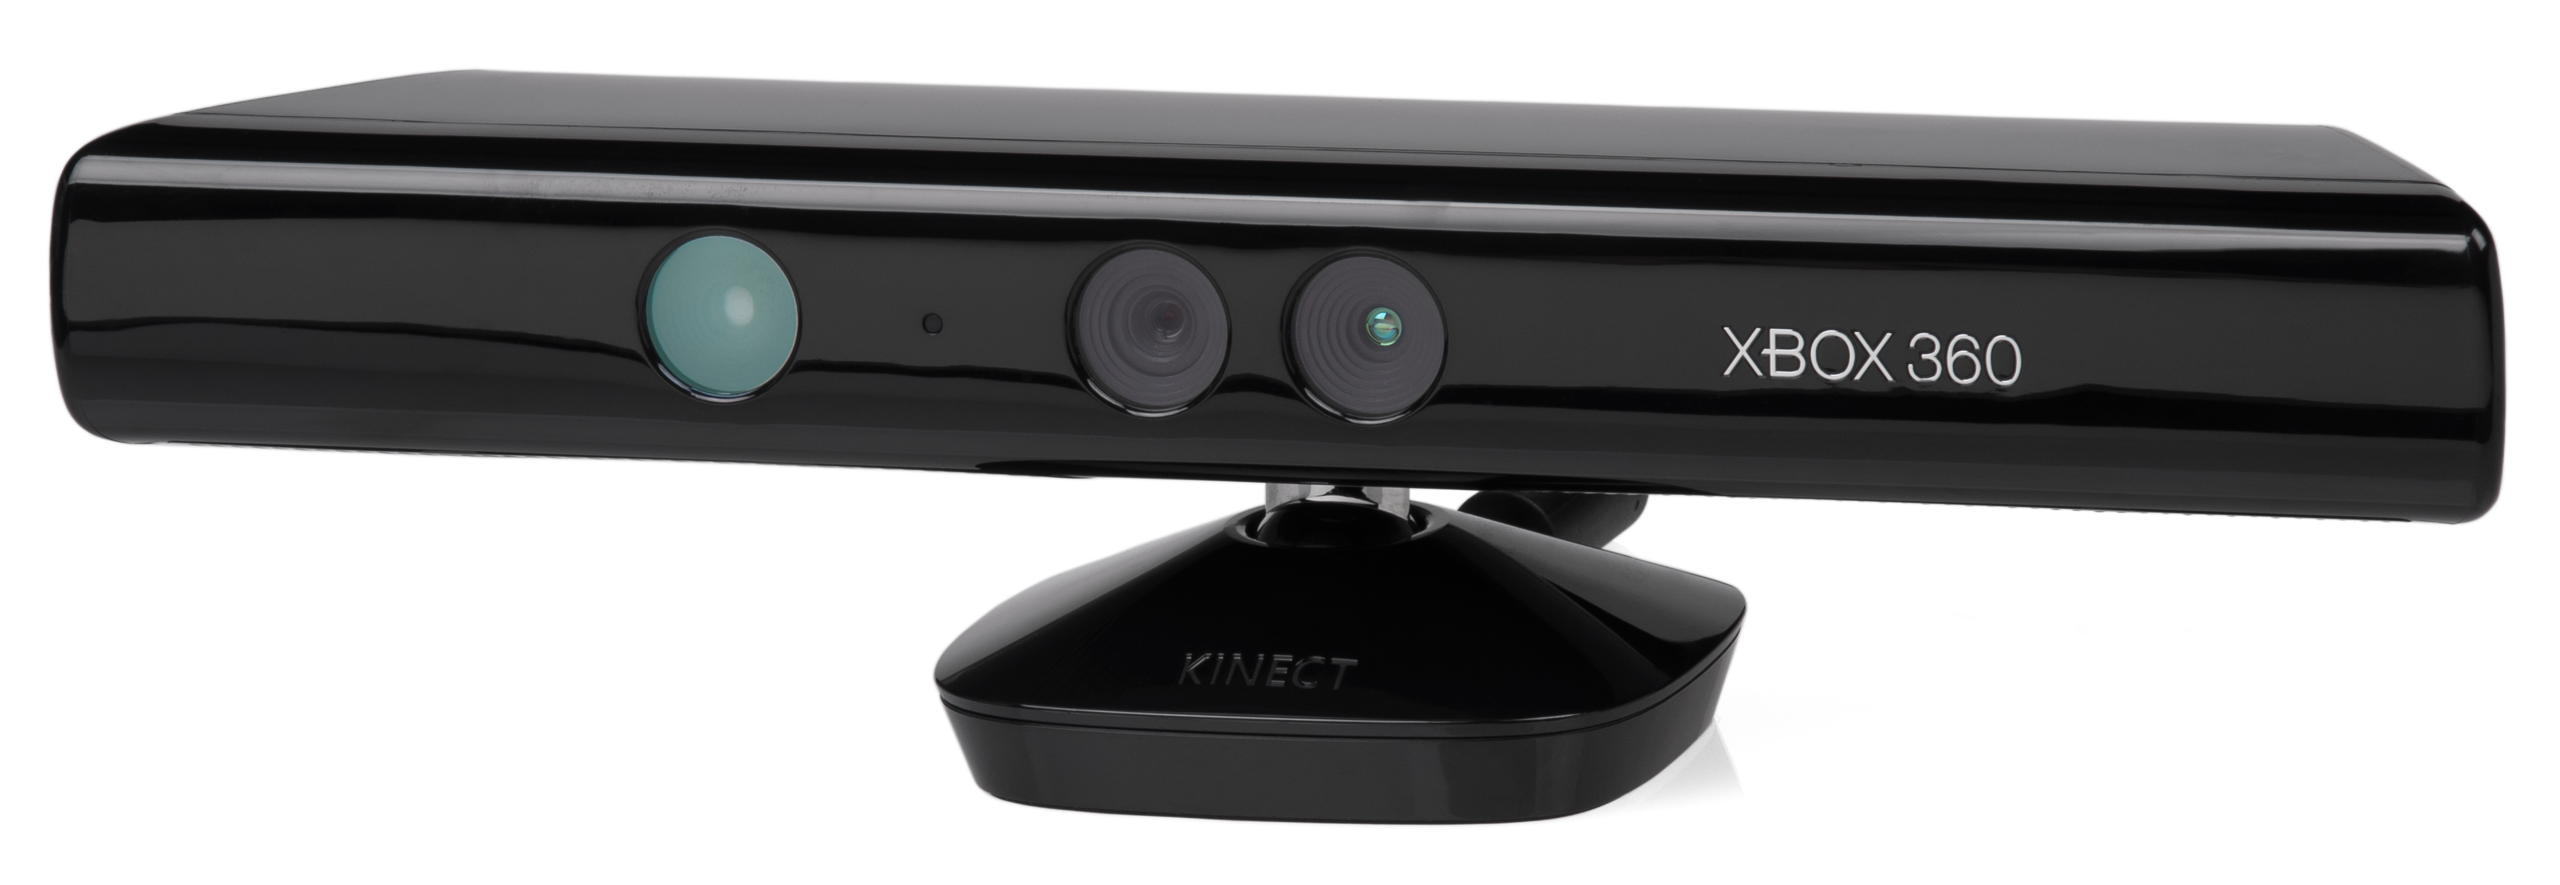
\includegraphics[width=0.45\linewidth]{figs/Xbox-360-Kinect-Standalone.png}(a)
	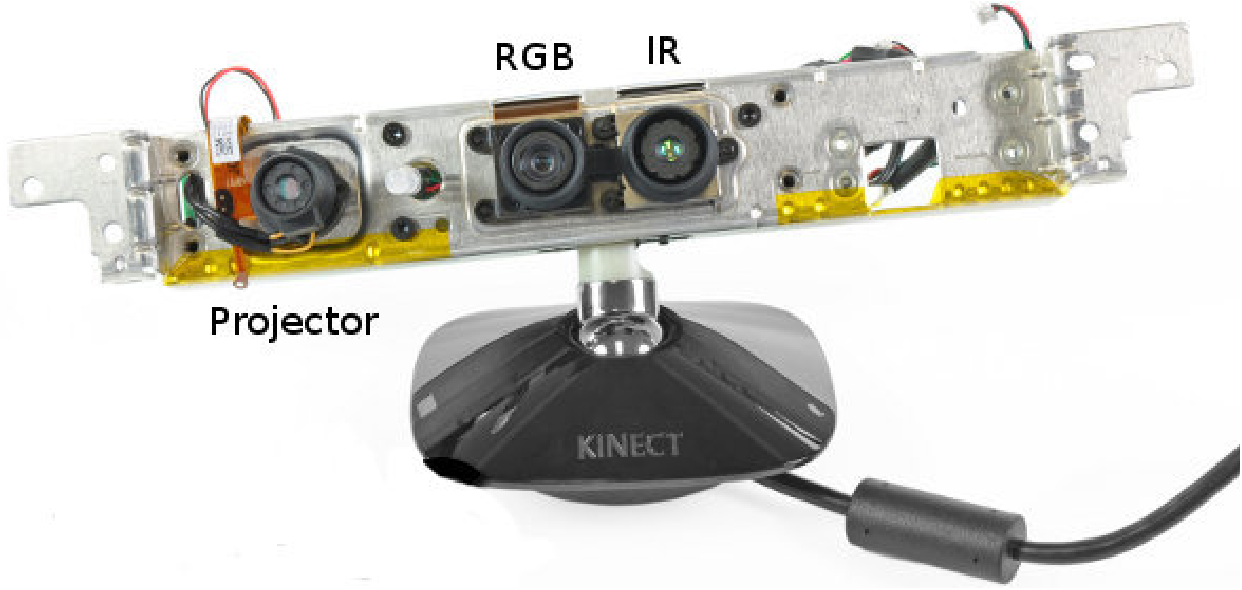
\includegraphics[width=0.45\linewidth]{figs/kinect-internals.pdf}(b)
 	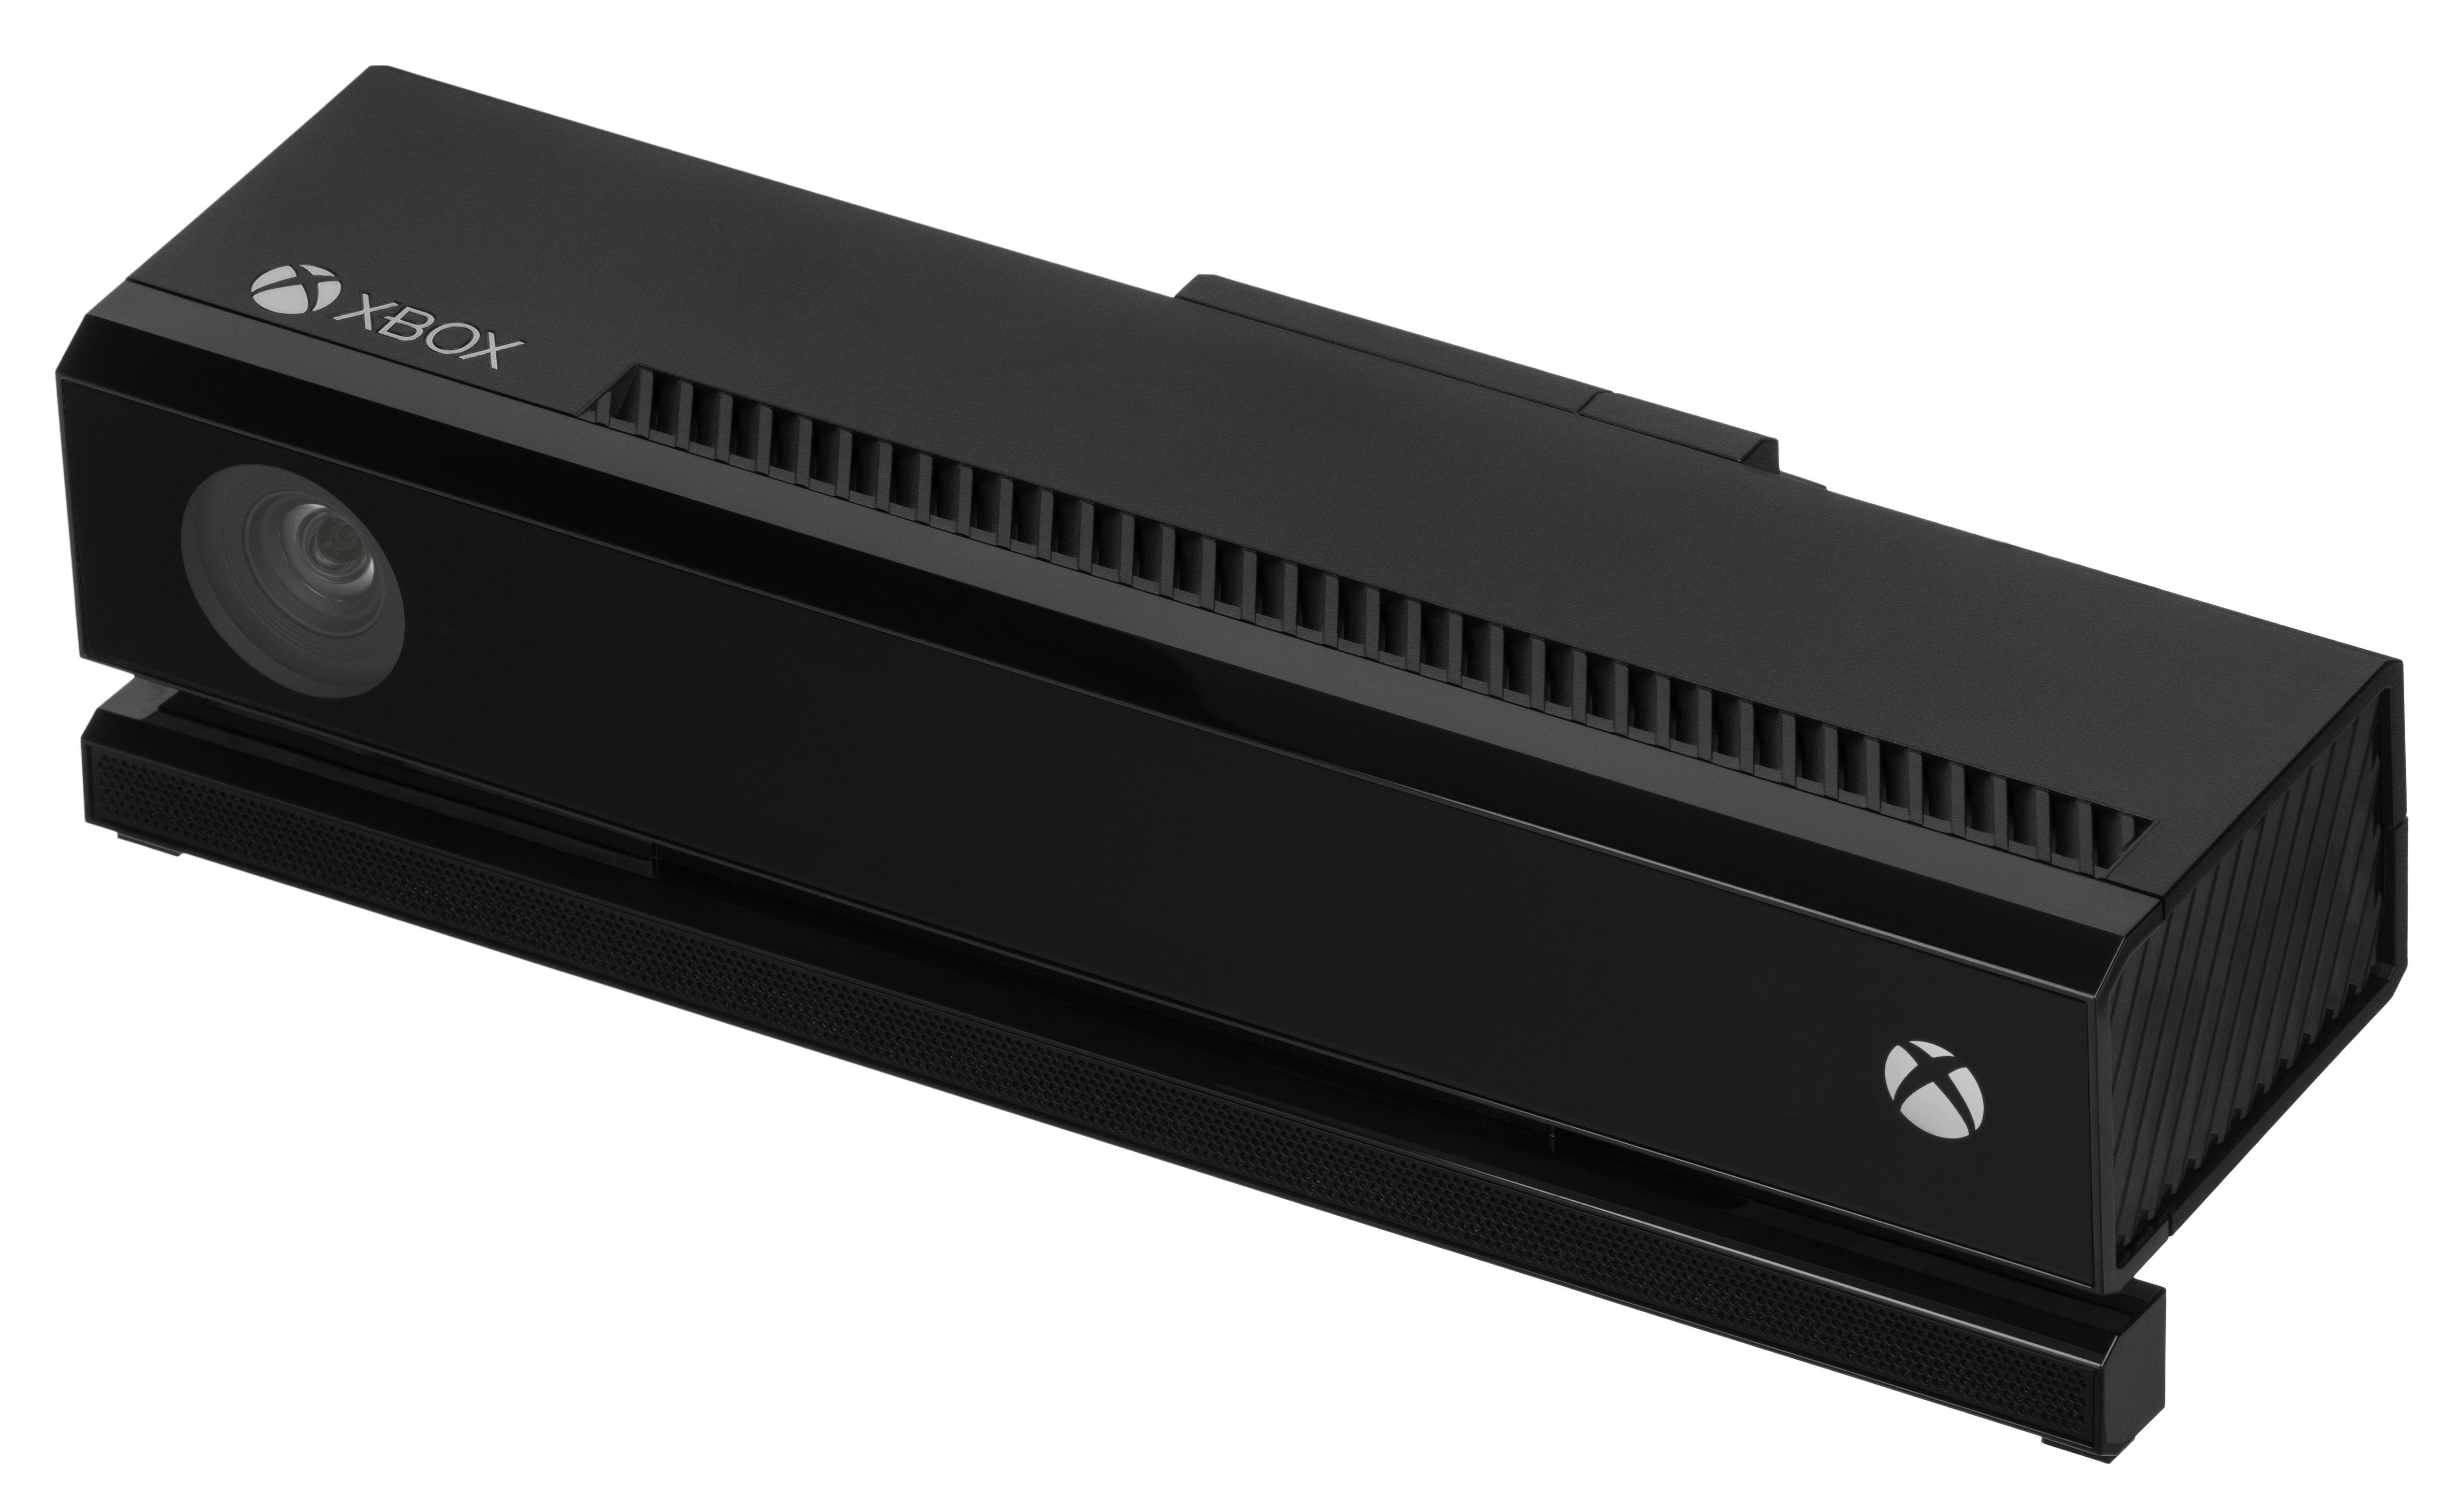
\includegraphics[width=0.45\linewidth]{figs/Xbox-One-Kinect.jpg}(c)
 	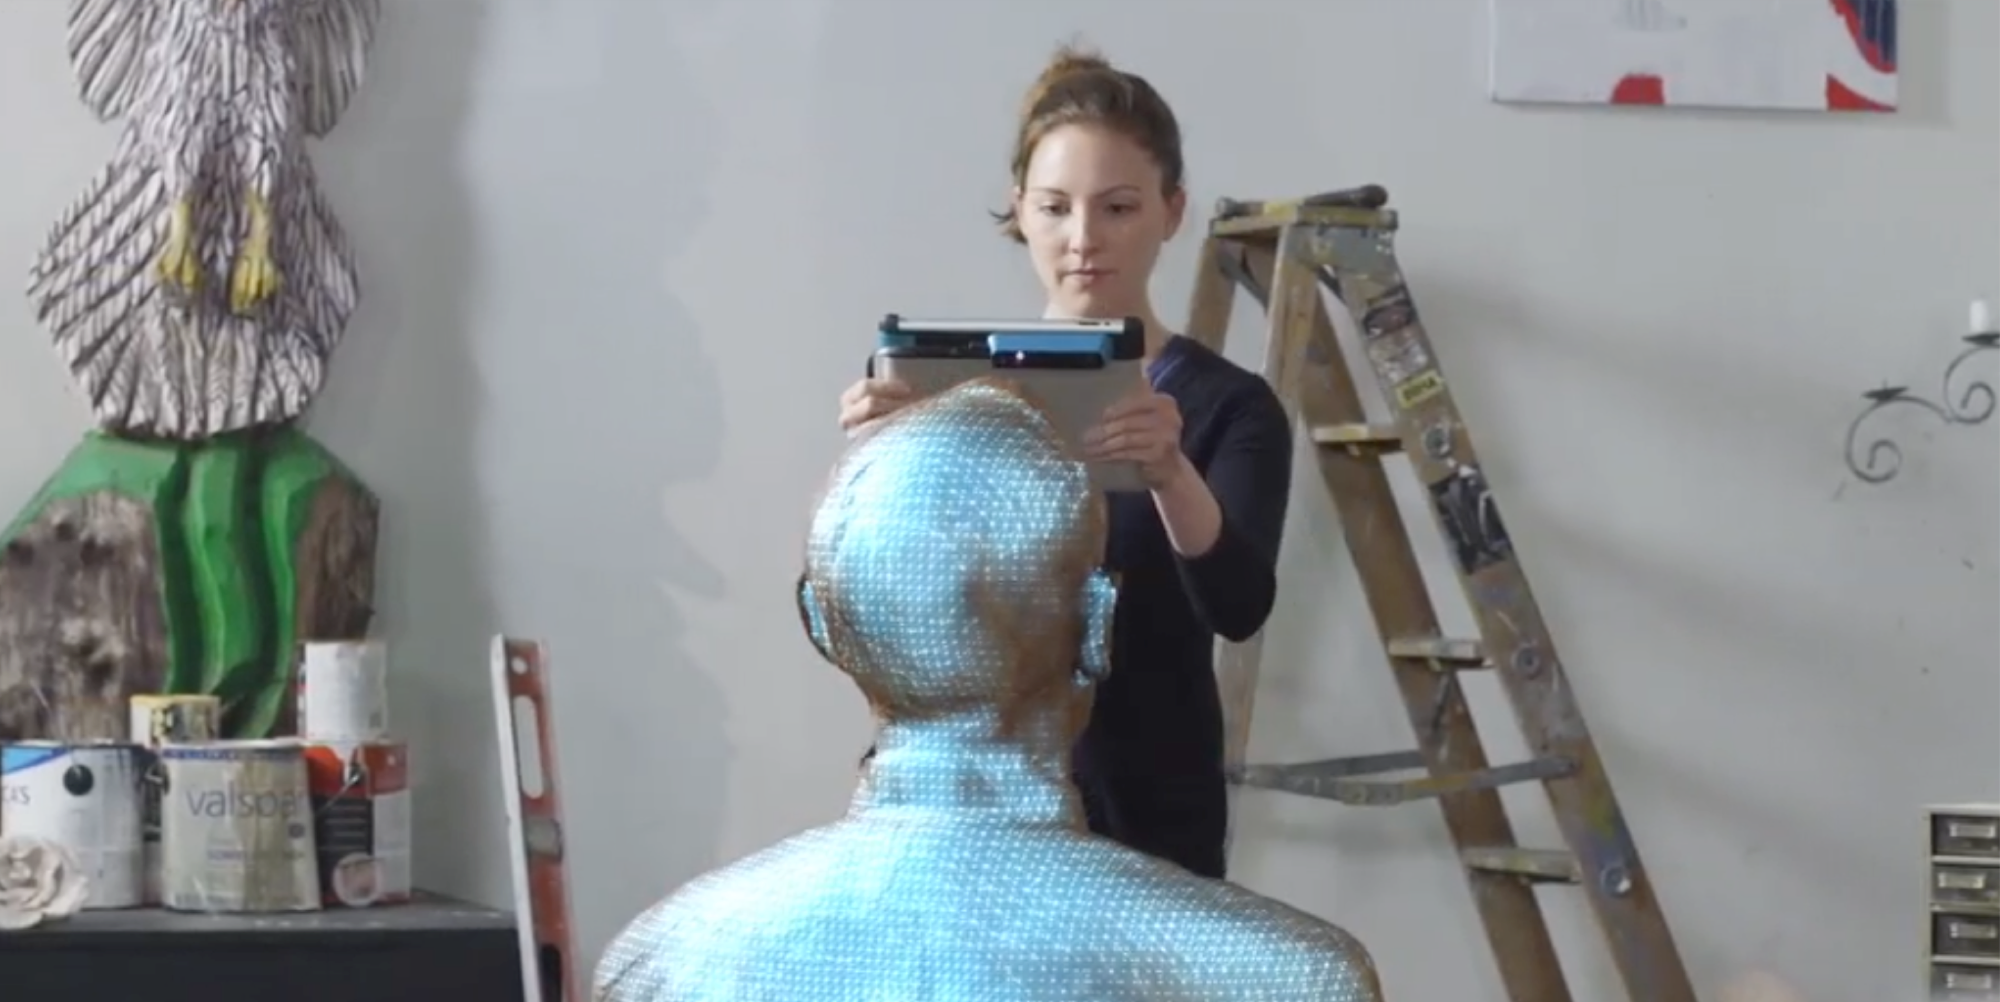
\includegraphics[width=0.45\linewidth]{figs/kinect-handheld1.png} (d)
	\caption{%
   Kinects de primeira geração (a) consistindo de câmeras e projetores
   infra-vermelho (b) e de segunda geração, consistindo de tecnologia ToF (c). 
   Ambos os kinects são largamente utilizados para escaneamento em tempo real, 
   formando a base de escaneadores manuais (d), porém nem sempre são úteis para 
   preservação detalhada de patrimônio. Um dos objetivos deste
   projeto é explorar os limites desta tecnologia.
	}\label{fig:kinect}
\end{figure}

A preservação de patrimônio tem sido realizada tradicionalmente com escaneadores
dedicados de alto custo, como no famoso projeto de escaneamento \emph{in situ} da escultura
David, chamado \emph{Digital Michelangelo}~\cite{levoy2000digital},
Figura~\ref{fig:david}.  O projeto teve início em 1992 e tem como objetivo a
utilização de escaneadores a \emph{laser} de profundidade (\emph{Rangefinder Scanners}),
aliado a algoritmos que combinam diferentes profundidades e cores da imagem,
para realizar uma digitalização da parte externa e da superficie de forma
acurada da estátua de David. Note-se, porém, que esse método pode ser utilizado em diferentes
objetos no mundo real, como partes de máquinas, artefatos culturais e na
indústria de video games, por exemplo.  Para as partes mais detalhadas, foi
utilizado um escaneador de menor escala que faz uma pequena triangulação com
laser de profundidade.

Mais recentemente, pode-se considerar tecnologias mais acessíveis, similares às
de altíssimo custo do projeto Digital Michelangelo e popularizadas na última
década pela indústria de entretenimento, notadamente pelo projeto
Natal/Kinect~\cite{smisek20133d,wang2015research}. A reconstrução usando-se Kinect (de
primeira ou segunda geração) usando software atual de super-resolução, é
inferior à de um sistema a \emph{laser} de alta qualidade, sendo, porém de baixo custo
e muito mais versátil devido ao sistema de aquisição manual e a software
amplamente utilizado e desenvolvido~\cite{wang2015research},
Figura~\ref{fig:rec3d:comparacao}.

% Seria de grande interesse explorar os dois paradigmas supracitados
% para avaliar as possibilidades disponíveis no estado da arte de reconstrução 3D
% para o escaneamento de baixo custo para a preservação de Patrimônio. O que se
% pode atingir com apenas uma filmagem de esculturas realizada por um smartphone,
% sem calibração prévia e \emph{in situ}, ou seja, sem ambiente controlado?  Como
% esta recontrução se compara nos dias de hoje com a reconstrução realizada por um
% escaneador padrão baseado em Kinect?

\begin{figure}[!h]
	\centering
	%   \includegraphics[width=1.0\linewidth]{figs/3d-curve-sketch/system-diagram.eps}
	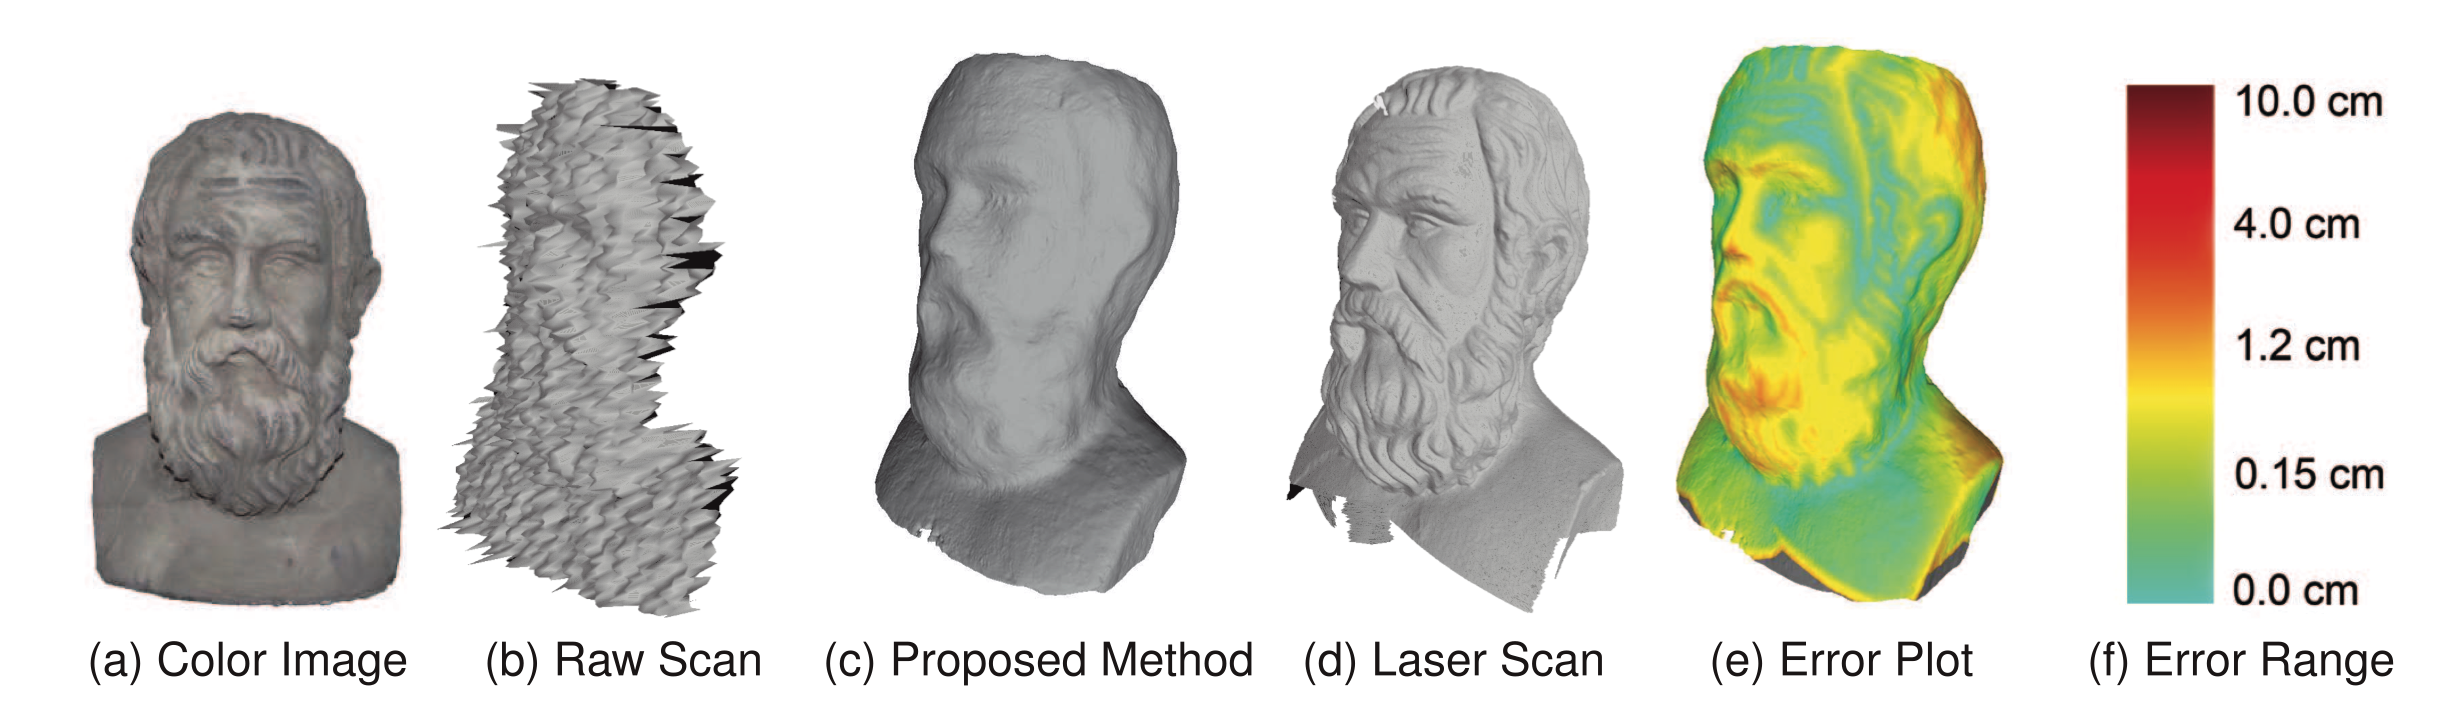
\includegraphics[width=1\linewidth]{figs/kinect-vs-usual.png}
	\caption{%
    A reconstrução usando-se Kinect (de primeira ou segunda geração) usando
    software atual de super-resolução (c) fornece precisão similar a um sistema estéreo de média
    resolução, inferior um sistema a \emph{laser} de alta qualidade (d) porém de baixo custo e
    muito mais versátil~\cite{wang2015research}.
	}\label{fig:rec3d:comparacao}
\end{figure}

\begin{figure}[!h]

\centering

\subfloat[]{\label{fig:davida}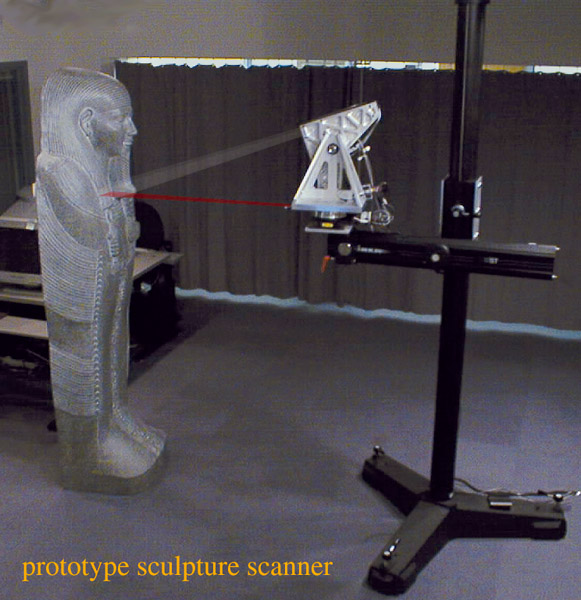
\includegraphics[height=0.38\linewidth]{figs/Proto+Inka+Egypt_light-s.jpg}}
% \vspace{2ex}
\subfloat[]{\label{fig:davidb}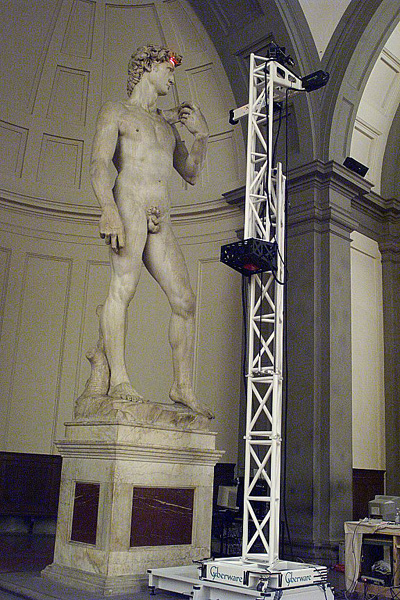
\includegraphics[height=0.38\linewidth]{figs/gantry-with-david-s.jpg}}\\
\subfloat[]{\label{fig:davidc}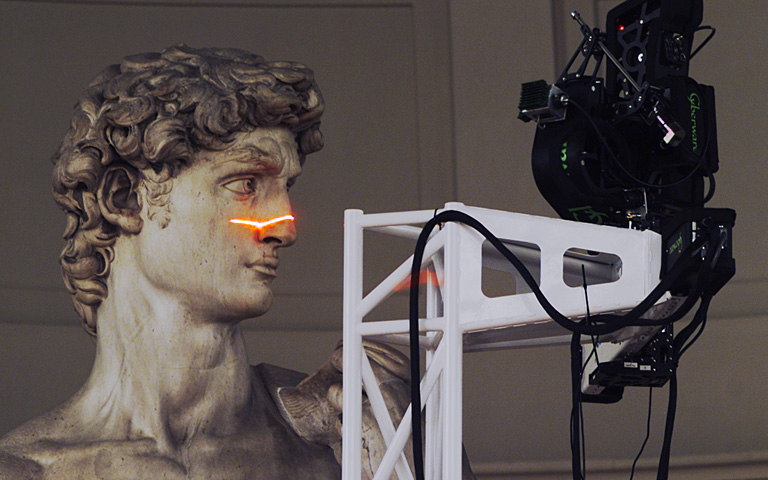
\includegraphics[height=0.25\linewidth]{figs/scanner-head-and-david-head-s.jpg}}
% \vspace{2ex}
\subfloat[]{\label{fig:davidd}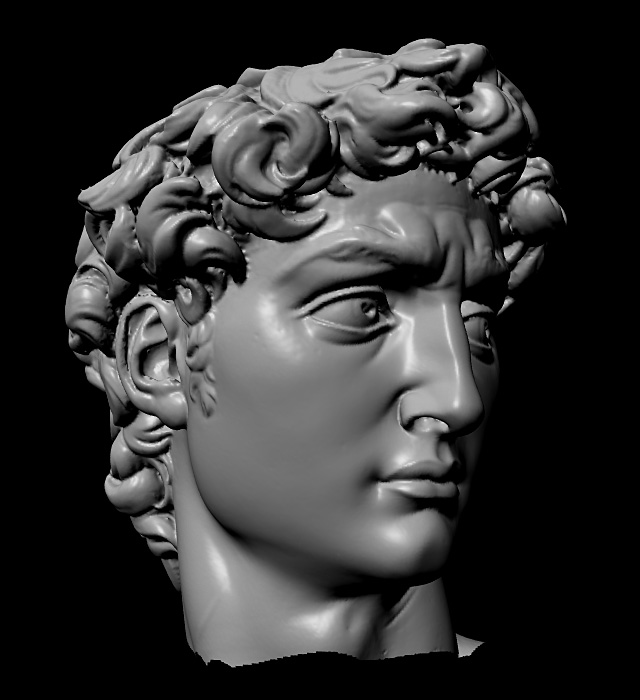
\includegraphics[height=0.25\linewidth]{figs/david-classic-leftlight-s.jpg}}
\caption{%
  Protótipo do escaneador a \emph{laser} do projeto clássico~\emph{Digital
  Michaelangelo}. Em (a), um objeto típico escaneado por um sistema inicial foi uma réplica em tamanho real
   de um sarcófago egípcio. O escaneador foi reconfigurado para objetos maiores, pois 
   a escultura David possui 517 centímetros (b); tabém foi reconfigurado para a cabeça,  
   para girar em 90 graus, que faz o \emph{laser}
   rotacionar da posição horizontal para a vertical e em torno da
   cabeça como um todo (c). Cerca de 100 \emph{scans}
   diversas posições foram alinhados automaticamente por um algoritmo 
   ICP (\emph{iterated-closest-points}). Após uma otimização global para minimizar erros 
   de alinhamento toda a estátua, usa-se um algoritmo VRIP (\emph {volumetric
   range image processing}) (d)~\cite{levoy2000digital}}.
  \label{fig:david}
\end{figure}

\subsection*{O Jardim do Nêgo, Nova Friburgo}
no caso de Nova Friburgo, há a necessidade redobrada de preservação de
patrimônio a céu aberto, em especial devido às chuvas e deslizamentos inerentes à região.  o
jardim do nêgo consiste em grandes esculturas em encostas, cobertas por um tapete de
vegetação, as quais desfrutam de grande reconhecimento regional e internacional~\cite{jardimdonego:theguardian},
Figura~\ref{fig:esculturas}.

\begin{figure} [!h]
	\centering
	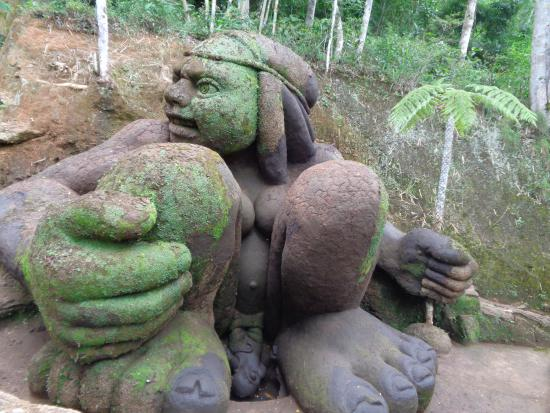
\includegraphics[height=0.23\linewidth]{figs/jardim-do-nego.jpg}
	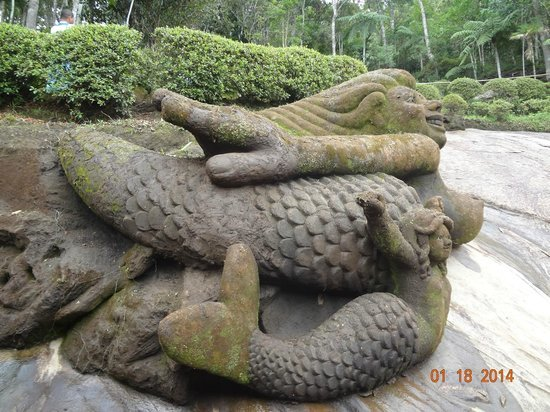
\includegraphics[height=0.23\linewidth]{figs/jardim-do-nego22.jpg}
	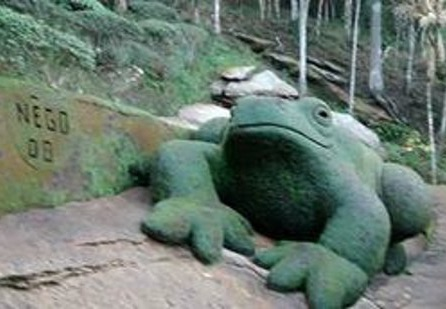
\includegraphics[height=0.23\linewidth]{figs/jardim-do-nego32-small.jpg}
	\caption{Algumas esculturas do Jardim do Nêgo~\cite{JardimDoNego:TheGuardian}}\label{fig:esculturas}
\end{figure}


% \begin{figure} [!h]
% 	\centering
% 	%   \includegraphics[width=1.0\linewidth]{figs/3d-curve-sketch/system-diagram.eps}
% 	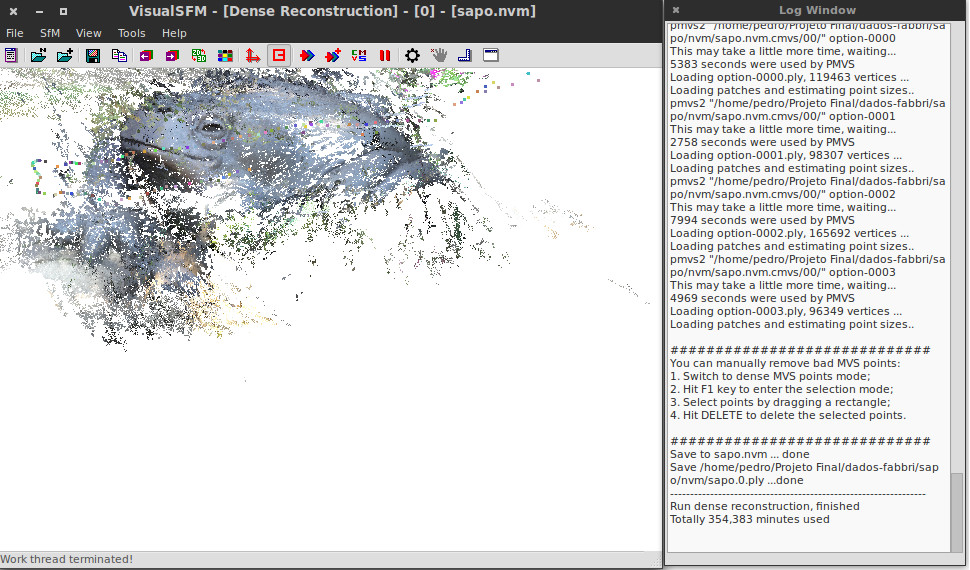
\includegraphics[width=1\linewidth]{figs/rec3d.jpg}
% %	\includegraphics[width=0.95\linewidth]{figs/rec3d-curves-pmvs.pdf}
% 	\label{fig:rec3d}
% 	\caption{A reconstrução usando-se apenas imagens, sem controle de aquisição, 
% 	   como em um vídeo de um smartphone filmado em torno do objeto, fornece uma
% 	   nuvem de pontos, que pode ser
% 	   densificada~\cite{snavely2010bundler,wu2011visualsfm,furukawa2007dense,mve}, ou
% 	   atribuída de
% 	   curvas~\cite{Usumezbas:Fabbri:Kimia:ECCV16,Fabbri:Kimia:IJCV2016,Fabbri:Kimia:CVPR10,Fabbri:Giblin:Kimia:ECCV12}, de forma a preservar a resolução
% 	   em áreas de alto conteúdo informativo. Tais representações estão sendo
% 	   atualmente unificadas na pesquisa da área. Este projeto propõe explorar os
% 	   limites da reconstrução 3D usando-se apenas imagens, no contexto de
% 	   preservação de patrimônio.}
% \end{figure}


Idealizado e criado por Geraldo Simplicio (Nêgo), artista cearense que mora no
local a mais de 30 anos, e que ganhou notoriedade por suas esculturas de barro,
com traços singulares e técnicas únicas. Hoje, trabalha para reconstruir o
Jardim após a tragédia de 2011 na região serrana, onde algumas estruturas foram
destruídas. Portanto, com o consentimento do Nêgo, surgiu a motivação desta
pesquisa: além de explorar métodos de reconstrução, também tem o objetivo de
ajudar a criar sistemas completos para eternizar um patrimônio que é reconhecido
no mundo todo.

A preservação das esculturas do Jardim do Nêgo se mostra um desafio à pesquisa em
recontrução 3D, pois apresentam curvas bem delineadas, que são 
representadas de maneira suavizada e empobrecida por métodos convencionais.
Algumas esculturas apresentam pouca textura, com apenas um leve padrão de musgo.
Seria de grande interesse avaliar o potencial de técnicas atuais de
reconstrução 3D geral que não exigem controle preciso de aquisição, as quais têm seu código fonte
disponível na internet.

\newpage

\section{Objetivos}\label{sec:objetivos}

Pretende-se, ao longo deste projeto, ganhar experiência com técnicas
modernas de reconstrução 3D fotogramétrica, no contexto de uma aplicação
bem-definida de preservação de patrimônio. 
% A entrada do sistema deverá ser um
% conjunto de vídeos realizados por câmeras de baixo custo, ou um conjunto de
% escaneamentos realizados por escaneadores à mão de baixo custo baseados em Kinect.

O objetivo concreto é explorar as tecnologias supracitadas para
desenvolver um esquema de escaneamento de patrimônio usando software aberto, câmeras e
escaneadores de baixo custo, representando o estado da arte em reconstrução 3D sem
restrições de aquisição. Perguntas fundamentais a serem respondidas são: que
nível de detalhe, facilidade e precisão se pode obter usando-se apenas imagens e software
aberto? É possível utilizar escaneadores de baixo custo baseados em Kinect com
melhorias significativas em termos de qualidade, conveniência ou tempo de
processamento?  Quais são as restrições desses sistemas? Seria útil, na prática,
uma reconstrução de curvas para auxiliar na reconstrução de nuvem de pontos e de
superfícies densas? Onde o estado da arte deve ser avançado de forma a permitir
uma solução mais conveniente e completa para a preservação de patrimônio?

O principal objetivo em termos de pesquisa científica será comparar as
diferentes abordagens do estado da arte disponíveis para reconstrução 3D e
explicitar suas limitações práticas.

\section*{Organização deste manuscrito}

Este trabalho foi estruturado da seguinte maneira: Introduzimos
métodos baseados em reconstrução a \emph{laser} no Capítulo~\ref{cap:laser},
apresentando, de uma maneira mais técnica, o projeto \emph{Digital
Michelangelo} na Seção~\ref{sec:David}, que foi um dos pioneiros na técnica de
conservação de acervos culturais. No próximo Capítulo~\ref{cap:kinect},
discutimos o uso do Kinect, da Microsoft, no que tange à calibração do sistema
para o uso em tecnologias \emph{Structure from Motion}.  Adiante, no
Capítulo~\ref{cap:pontosdeinteresse}, abordaremos o tema central do trabalho:
técnicas de reconstrução baseadas em fotogrametria, com o emprego de dois
softwares, o MVE~\ref{sec:mve} e o VisualSfM~\ref{sec:visualsfm} e seus
respectivos funcionamentos. Ao final, apresentamos experimentos e conclusões
do trabalho, bem como sugestões para implementações e trabalhos futuros.

% O trabalho foi estruturado da seguinte maneira: previamente introduzimos os métodos baseados em pontos de interesse no Capítulo~\ref{sec:pontosdeinteresse}, destacando suas funcionalidades. No Capítulo~\ref{sec:denserecon} discutimos e aprofundamos o  funcionamento de cada algoritmo de reconstrução densa empregados, apresentando e debatendo, comparativamente, pontos à favor e contra; O Capítulo~\ref{sec:kinect} é apresentada a técnica de reconstrução utilizada nos  {\it Kinects}, da Microsoft; Com isso, temos o  Capítulo~\ref{sec:visualsfm}, que é dedicado à ferramenta gráfica utilizada para a obtenção dos resultados (VisualSfM) dos algoritmos de reconstrução densa utilizados. Finalmente, apresentamos os resultados e conclusões do trabalho, bem como sugestões para implementações e trabalhos futuros.
%Este trabalho está organizado da seguinte forma: discutimos as técnicas de
%extração de curva sem aprendizagem de máquina supervisionada no
%Capítulo~\ref{sec:cfrag:extraction}. No Capítulo~\ref{sec:learning:chapter},
%discutimos maneiras pelas quais essas técnicas podem ser melhoradas
%usando dados de treinamento anotados por humanos como entrada para uma
%aprendizagem de máquina geométrica de topologia e semântica de fragmentos de
%curva. A maior parte deste material é
%de~\cite{Guo:etal:CVPR14,Guo:etal:PAMI2017:submitted,Tamrakar:PHD:2008}, com esclarecimentos
%substanciais e comentários sobre as questões relativas aos nossos objetivos
%específicos. No Capítulo~\ref{sec:generic:datasets}, apresentamos o processo de
%captura de dados confiáveis (\emph{ground-truth}), comparando os conjuntos de dados anteriores com o problema proposto
%neste trabalho para a água. Nos capítulos restantes, apresentamos e discutimos
%nossos resultados para vários vídeos em tanques de água. Partes deste trabalho
%foram apresentadas em~\cite{Fabbri:WaterWaves2016,Fabbri:WaterWaves2017,Souza:Fabbri:WaterWaves2017}.

%======================================================================================

%\input{cfragextract}
%\input{learningcurves}
%\input{datasets}
%\chapter{Experimentos}\label{sec:experiments}
%======================================================================================
No presente trabalho, nos concentramos no objetivo proposto descrito na Seção~\ref{sec:objetivos}.

\section{Procedimento}
Primeiramente, filmamos algumas esculturas utilizando a câmera de um \emph{smartphone} convencional na resolução de 1920x1080 pixels. Esta filmagem foi realizada varrendo toda (ou maioria) da superfície da escultura em $360^{\circ}$ com o intuito de ter toda a escultura reconstruída \ref{fig:procedimentoscan}.
Após isso, fizemos mais alguns vídeos, pegando alguns pontos que possuíam mais detalhes e que, com uma única varredura, não era capaz de reproduzir uma boa reconstrução.

\begin{figure}[!h]
	\centering
	%   \includegraphics[width=1.0\linewidth]{figs/3d-curve-sketch/system-diagram.eps}
	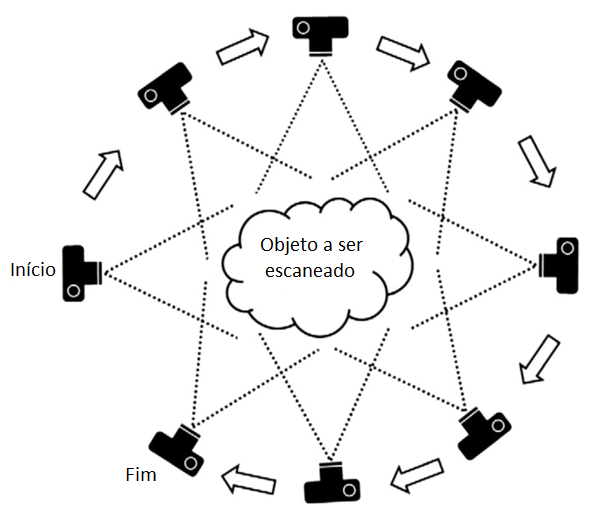
\includegraphics[width=0.4\linewidth]{figs/procedimentoscan.png}
	\caption{%
	Exemplo de como foi realizada a varredura da escultura
	%\cite{Cui:Theobalt:etal:PAMI2013,Pajdla:etal:ICCV2011}.
	}\label{fig:procedimentoscan}
\end{figure}

Com este material, foram feitos "cortes" em determinados \emph{frames} do vídeo, com atenção para não cortar em \emph{frames} muito juntos, pois aumentaria o número de correspondências ambíguas entre as imagens e com isso, o processamento da reconstrução demoraria mais. E não usar \emph{frames} muito distantes, que ocorreria o inverso: com menos correspondências, ficariam buracos (partes sem a informação necessária) na reconstrução, como descrito na Seção \ref{sec:mve}.

Com isso em mente, foram reconstruídas duas esculturas: empregando o VisualSfM, usamos um único vídeo, totalizando 197 imagens. %guerreiro, indio%
Com o MVE, utilizamos dois vídeos, que, ao cortá-los, totalizou cerca de 280 imagens. %sapo%

Além de esculturas ao ar livre, fizemos alguns testes em ambiente fechado, dentro de uma casa, por exemplo. Foi utilizado um objeto feito de cabaça (casca de abóbora) na qual possui uma superfície propícia (Lambertiana)~\cite{basri2003lambertian} para uma reconstrução.

Com o procedimento descrito anteriormente, a partir dos vídeos feitos, obtemos um total de 200 imagens em um vídeo superficial e mais 24 imagens mais detalhadas do objeto, ambos numa resolução de 1080x1920 pixels. E, para um mesmo conjunto de imagens, rodamos tanto o VisualSfM quanto o MVE.

\subsection{Resultados da reconstrução com o VisualSfM}

Seguindo o passo-a-passo de reconstrução do software, obtivemos os seguintes resultados, para a escultura de 197 imagens do Jardim do Nêgo.

\begin{table}[h!]
\caption{Tempos obtidos da reconstrução da escultura do Jardim do Nêgo usando o VisualSfM}
\label{tab:temposSfMJardimDoNego}
\begin{tabular}{|l|p{4.7cm}|}
\hline
Procedimento & Tempo (aprox.) \\ \hline
Carregamento de imagens & 10 segundos \\ \hline
Calcular pares correspondentes de \emph{features} & 6.643 segundos \\ \hline
Gerar a reconstrução esparsa do modelo & 220 segundos \\ \hline
Gerar a reconstrução densa do modelo & 1.385 segundos \\ \hline
\end{tabular}
\end{table}

Com as seguintes reconstruções~\ref{fig:reconstrucaoEsparsaIndioVisualSFM},~\ref{fig:reconstrucaoDensaIndioVisualSFM}.
Percebemos que foi gerada uma nuvem de pontos bem consistente, a partir da reconstrução esparsa do algoritmo PBA.
Por conta disso, nossa reconstrução 3D densa, empregando o MCBA/PMVS-2 obteve uma qualidade adequada para o conjunto de imagens usada.
%COLOCAR IMAGENS GUERREIRO AQUI%

\begin{figure}[!h]
	\centering
	%   \includegraphics[width=1.0\linewidth]{figs/3d-curve-sketch/system-diagram.eps}
	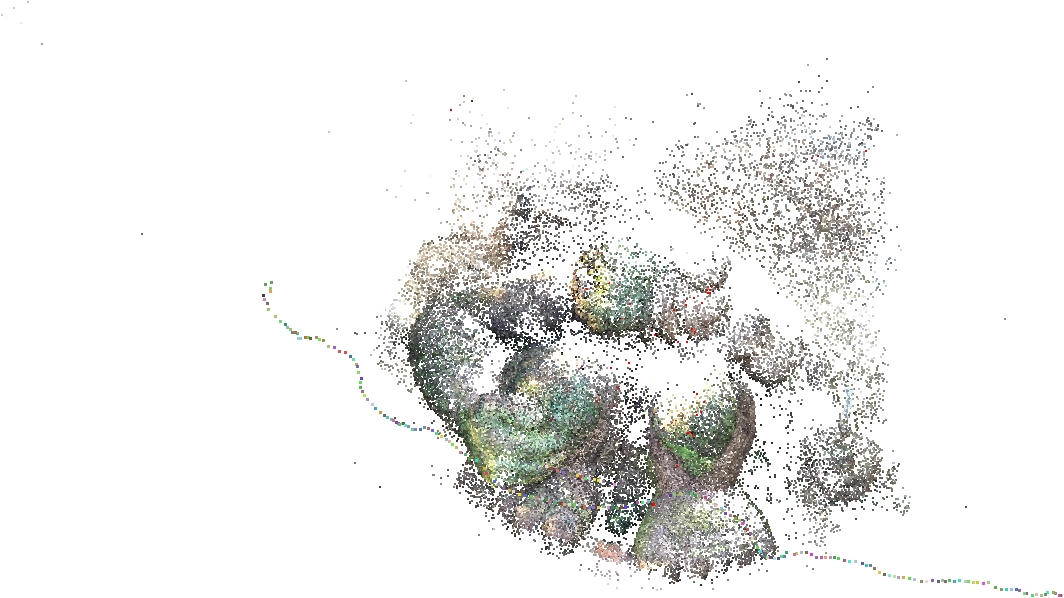
\includegraphics[width=0.9\linewidth]{figs/guerreiroEsparsa.jpg}
	\caption{%
	Reconstrução esparsa da escultura do Jardim do Nêgo no VisualSfM com 197 imagens.
	%\cite{Cui:Theobalt:etal:PAMI2013,Pajdla:etal:ICCV2011}.
	}\label{fig:reconstrucaoEsparsaIndioVisualSFM}
\end{figure}

\newpage

\begin{figure}[!h]
	\centering
	%   \includegraphics[width=1.0\linewidth]{figs/3d-curve-sketch/system-diagram.eps}
	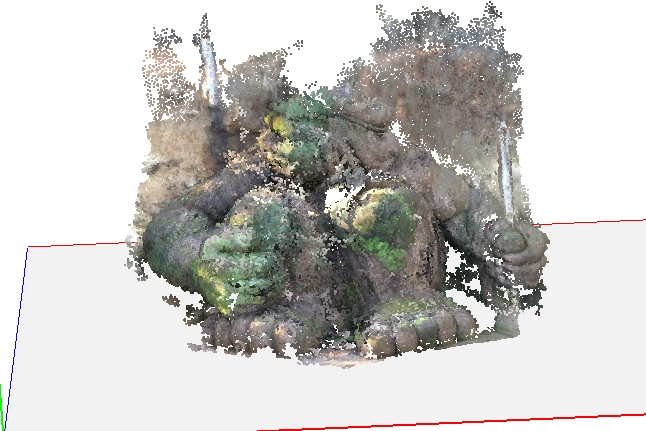
\includegraphics[width=0.40\linewidth]{figs/guerreirovisualsfmdmr.jpg}(a)
	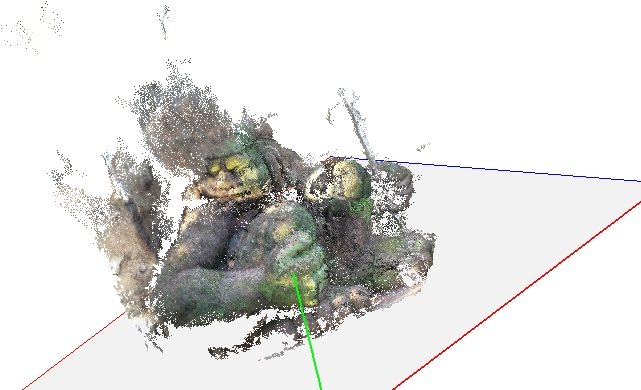
\includegraphics[width=0.50\linewidth]{figs/guerreirovisualsfmdmr2.jpg}(b)
	\caption{%
	Resultados da reconstrução densa da escultura do Jardim do Nêgo usando o VisualSfM, em dois ângulos diferentes (a) e (b).
	%\cite{Cui:Theobalt:etal:PAMI2013,Pajdla:etal:ICCV2011}.
	}\label{fig:reconstrucaoDensaIndioVisualSFM}
\end{figure}


%-------------------GALINHA A PARTIR DAQUI----------------------------------%

Com o objeto em ambiente fechado, conseguimos os resultados a seguir. 

Para o primeiro vídeo, convertido em 200 imagens:

\begin{table}[h!]
\caption{Tempos obtidos da reconstrução do objeto, com 200 imagens usando o VisualSfM}
\label{tab:temposSfM}
\begin{tabular}{|l|p{4.7cm}|}
\hline
Procedimento & Tempo (aprox.) \\ \hline
Carregamento de imagens & 50 segundos \\ \hline
Calcular pares correspondentes de \emph{features} & 9.540 segundos \\ \hline
Gerar a reconstrução esparsa do modelo & 135 segundos \\ \hline
Gerar a reconstrução densa do modelo & 1.416 segundos \\ \hline
\end{tabular}
\end{table}

A Figura~\ref{fig:reconstrucaoEsparsaVisualSFM} mostra o resultado da
reconstrução esparsa do algoritmo PBA. Não é tão nítida como na reconstrução
densa, Figura~\ref{fig:reconstrucaoDensaVisualSFM}, a quantidade de ruídos,
provenientes de outros objetos presentes na cena (o VisualSfM só identifica
objetos estáticos). Só é possível limpar a malha manualmente, pressionando a
tecla F1 e selecionando a área desejada para ser deletada. Não é muito prático,
pois podemos excluir alguns pontos importantes, o ideal seria fazer esta limpeza
por meio de programas externos.

\begin{figure}[!h]
	\centering
	%   \includegraphics[width=1.0\linewidth]{figs/3d-curve-sketch/system-diagram.eps}
	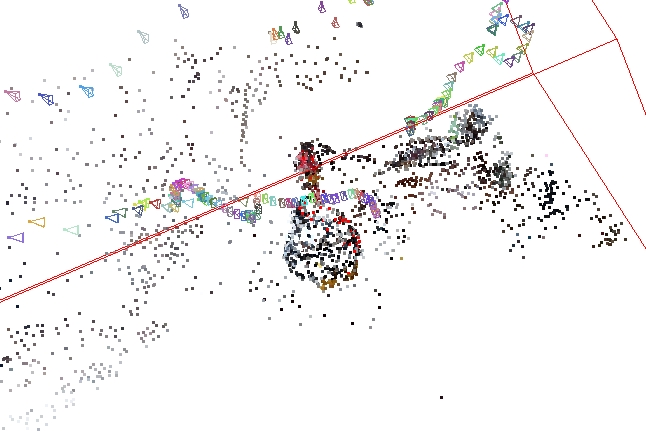
\includegraphics[width=0.5\linewidth]{figs/galinhasparsa.jpg}
	\caption{%
	Reconstrução esparsa do objeto no VisualSfM com 200 imagens.
	%\cite{Cui:Theobalt:etal:PAMI2013,Pajdla:etal:ICCV2011}.
	}\label{fig:reconstrucaoEsparsaVisualSFM}
\end{figure}

\begin{figure}[!h]
	\centering
	%   \includegraphics[width=1.0\linewidth]{figs/3d-curve-sketch/system-diagram.eps}
	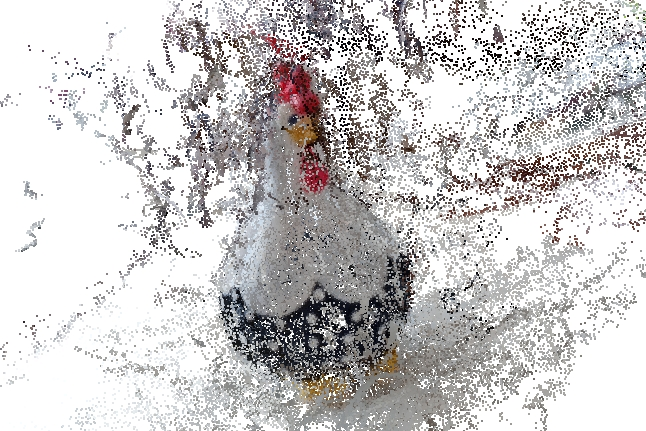
\includegraphics[width=\linewidth]{figs/galinhadense.jpg}
	\caption{%
	Reconstrução densa do objeto no VisualSfM com 200 imagens.
	%\cite{Cui:Theobalt:etal:PAMI2013,Pajdla:etal:ICCV2011}.
	}\label{fig:reconstrucaoDensaVisualSFM}
\end{figure}

Fizemos uma outra reconstrução, utilizando os dois vídeos (gerando 224 imagens). Caso usássemos um conjunto maior, o programa parava de funcionar por falta de memória, mesmo após ajustar parâmetros (como o número de vizinhos, número de \emph{cores} do processador, \emph{level} do PMVS, entre outros) para melhorar esse problema. Portanto, o experimento seguiu da forma:

\begin{table}[h!]
\caption{Tempos obtidos da reconstrução do objeto, com 224 imagens usando o VisualSfM}
\label{tab:temposSfM224}
\begin{tabular}{|l|p{4.7cm}|}
\hline
Procedimento & Tempo (aprox.) \\ \hline
Carregamento de imagens & 60 segundos \\ \hline
Calcular pares correspondentes de \emph{features} & 10.451 segundos \\ \hline
Gerar a reconstrução esparsa do modelo & 162 segundos \\ \hline
Gerar a reconstrução densa do modelo & 1920 segundos \\ \hline
\end{tabular}
\end{table}

Percebemos que não foi tão proveitoso (qualitativamente) usar mais imagens neste
caso, inclusive o algoritmo perdeu a referência do objeto e gerou um segundo
modelo na reconstrução esparsa,
Figura~\ref{fig:reconstrucaoEsparsaVisualSFM224}, e, consequentemente, na
reconstrução densa,
Figuras~\ref{fig:reconstrucaoDensaVisualSFM2241},~\ref{fig:reconstrucaoDensaVisualSFM2241:2} e~\ref{fig:reconstrucaoDensaVisualSFM2242}. O que gerou uma certa incoerência na reconstrução.

\begin{figure}[!h]
	\centering
	%   \includegraphics[width=1.0\linewidth]{figs/3d-curve-sketch/system-diagram.eps}
	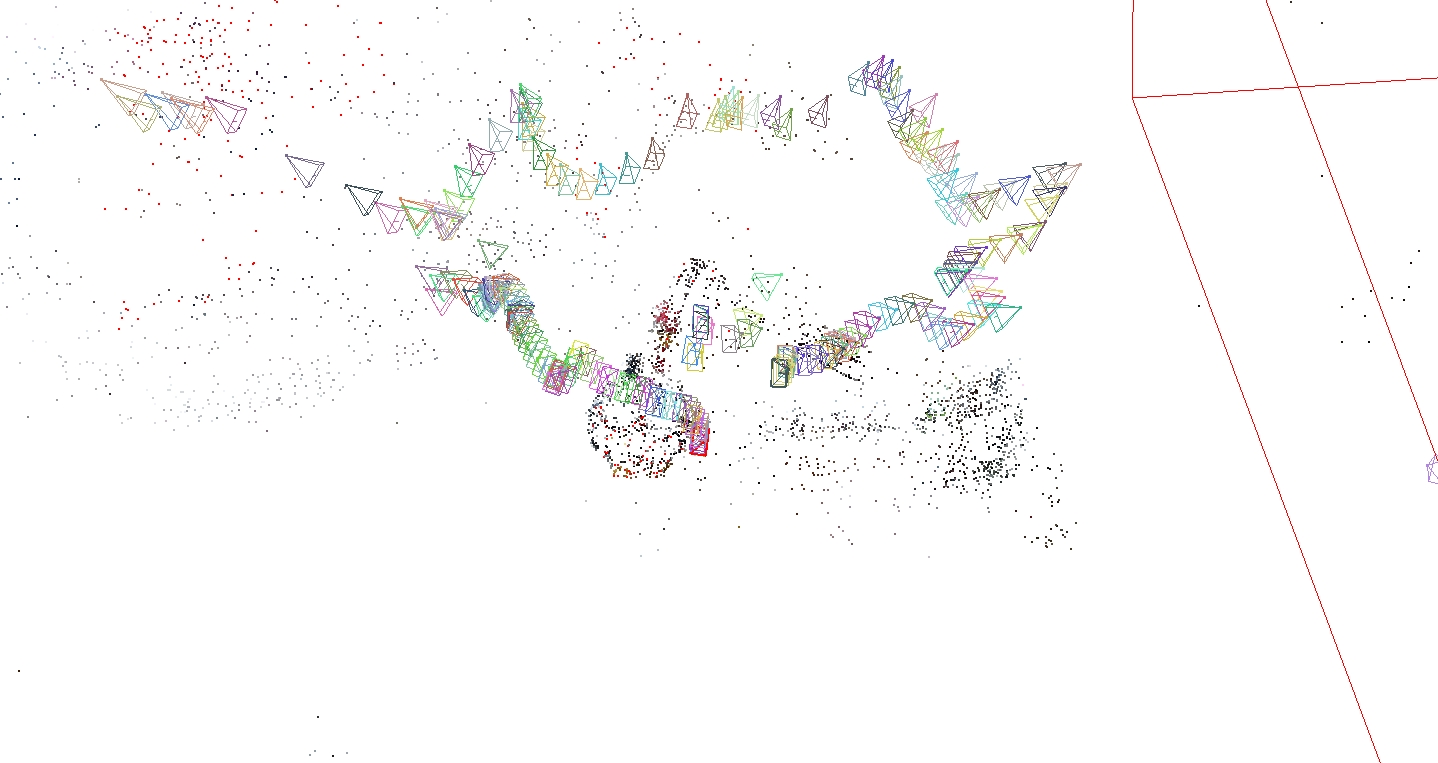
\includegraphics[width=\linewidth]{figs/perto_longe_esparsa.jpg}
	\caption{%
	Reconstrução esparsa do objeto com 224 imagens no VisualSfM.
	%\cite{Cui:Theobalt:etal:PAMI2013,Pajdla:etal:ICCV2011}.
	}\label{fig:reconstrucaoEsparsaVisualSFM224}
\end{figure}

\begin{figure}[!h]
	\centering
	%   \includegraphics[width=1.0\linewidth]{figs/3d-curve-sketch/system-diagram.eps}
	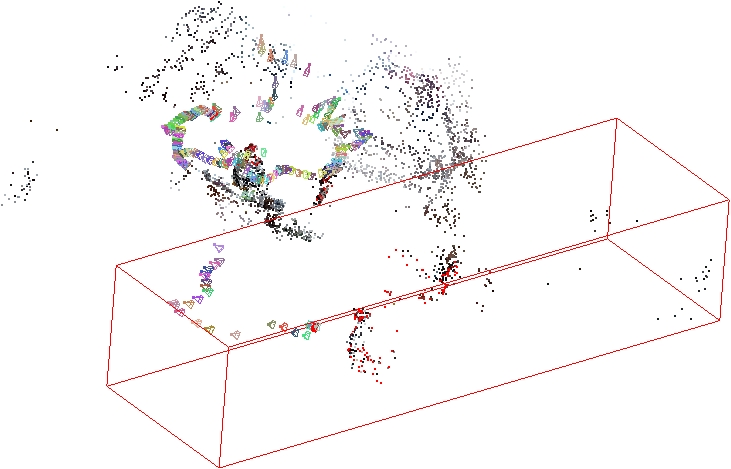
\includegraphics[width=\linewidth]{figs/perto_longe_esparsa_2.jpg}
	\caption{%
	Caso em que foram gerados dois modelos refletidos esparsos do objeto a partir
  do conjunto inicial de 224 imagens, provavelmente, proveniente da falta de
  informações para estimar as câmeras.
	%\cite{Cui:Theobalt:etal:PAMI2013,Pajdla:etal:ICCV2011}.
	}\label{fig:reconstrucaoEsparsaVisualSFM224:2}
\end{figure}

\begin{figure}[!h]
	\centering
	\subfloat[]{\label{fig:reconstrucaoDensaVisualSFM2241}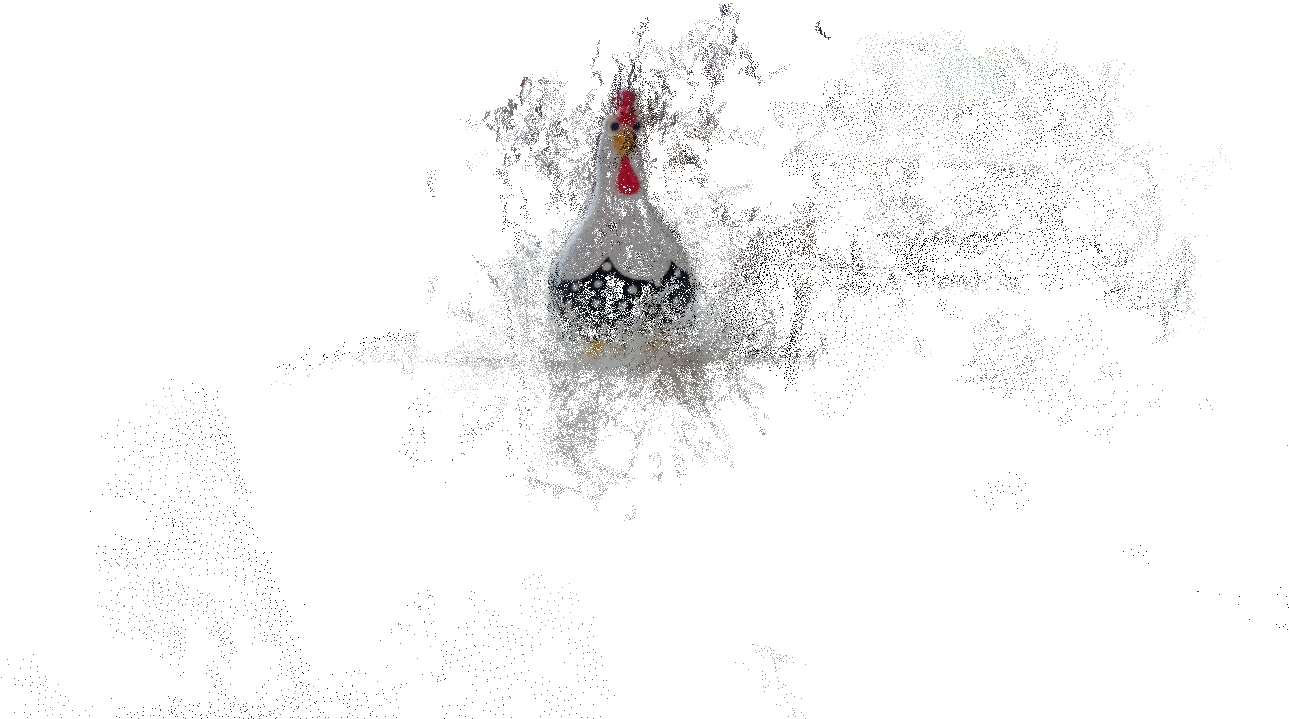
\includegraphics[width=0.5\linewidth]{figs/galinhadense224.jpg}}
	\subfloat[]{\label{fig:reconstrucaoDensaVisualSFM2242}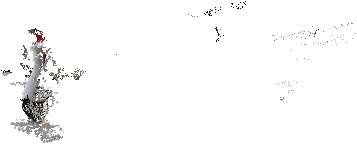
\includegraphics[width=0.5\linewidth]{figs/galinhavisualsfm224.jpg}}
	\caption{Reconstruções densas do primeiro (a) e do segundo (b) modelo do objeto no VisualSfM com 224 imagens.
	}
\end{figure}

%------------------ACABOU SFM---------------------------------------------%

\subsection{Resultados da reconstrução com o MVE}

A utilização do software é bem intuitiva, seja por linha de comando ou pela interface gráfica (neste modo, fica mais fácil visualizar cada etapa da reconstrução). Amplamente configurável, podendo escolher a vizinhança, escala, manter o mapa de profundidade, ver os dados \emph{EXIF} de cada imagem, dentre outras configurações.

Entretanto, para a aplicação proposta neste projeto, não é muito interessante, visto que ele utiliza a informação das câmeras, inseridas nas imagens (\emph{EXIF}) e como as imagens empregadas na reconstrução são, tecnicamente, vídeos cortados em determinados \emph{frames}, não é possível obter a informação das câmeras~\ref{fig:mveexif}. Logo o software não tem tanta aplicabilidade neste caso, pois pode recair no problema dos parâmetros padrões adotados para as câmeras não serem bons o suficiente para estes conjuntos de dados. A menos que sejam tiradas fotos sequenciais de alguma escultura ou objeto que se deseja gerar a reconstrução densa, pois dessa forma, as informações necessárias das câmeras estarão armazenadas.

\begin{figure}[!h]
	\centering
	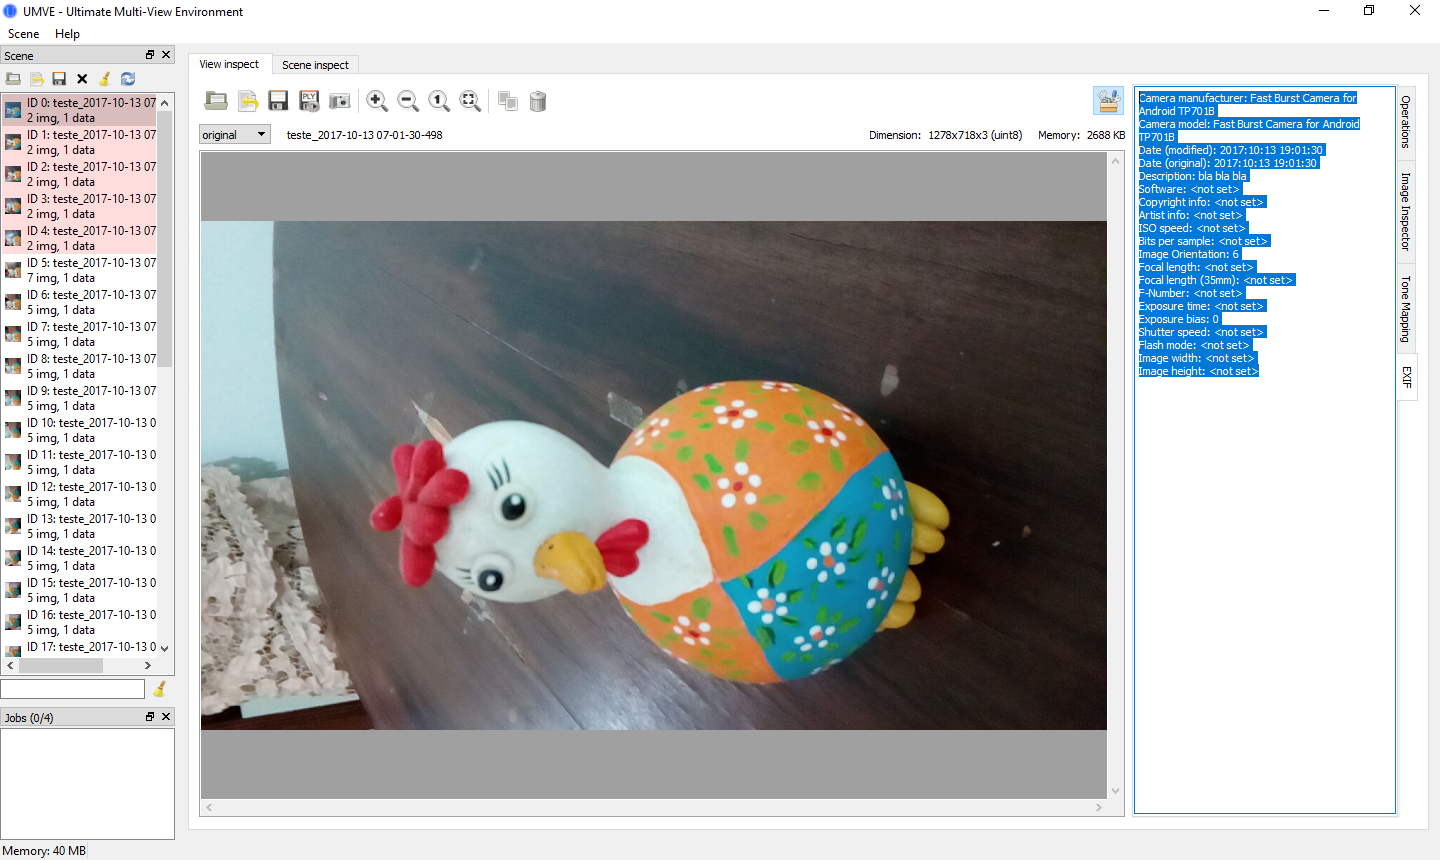
\includegraphics[width=0.461\linewidth]{figs/exifumve.png}(a)
	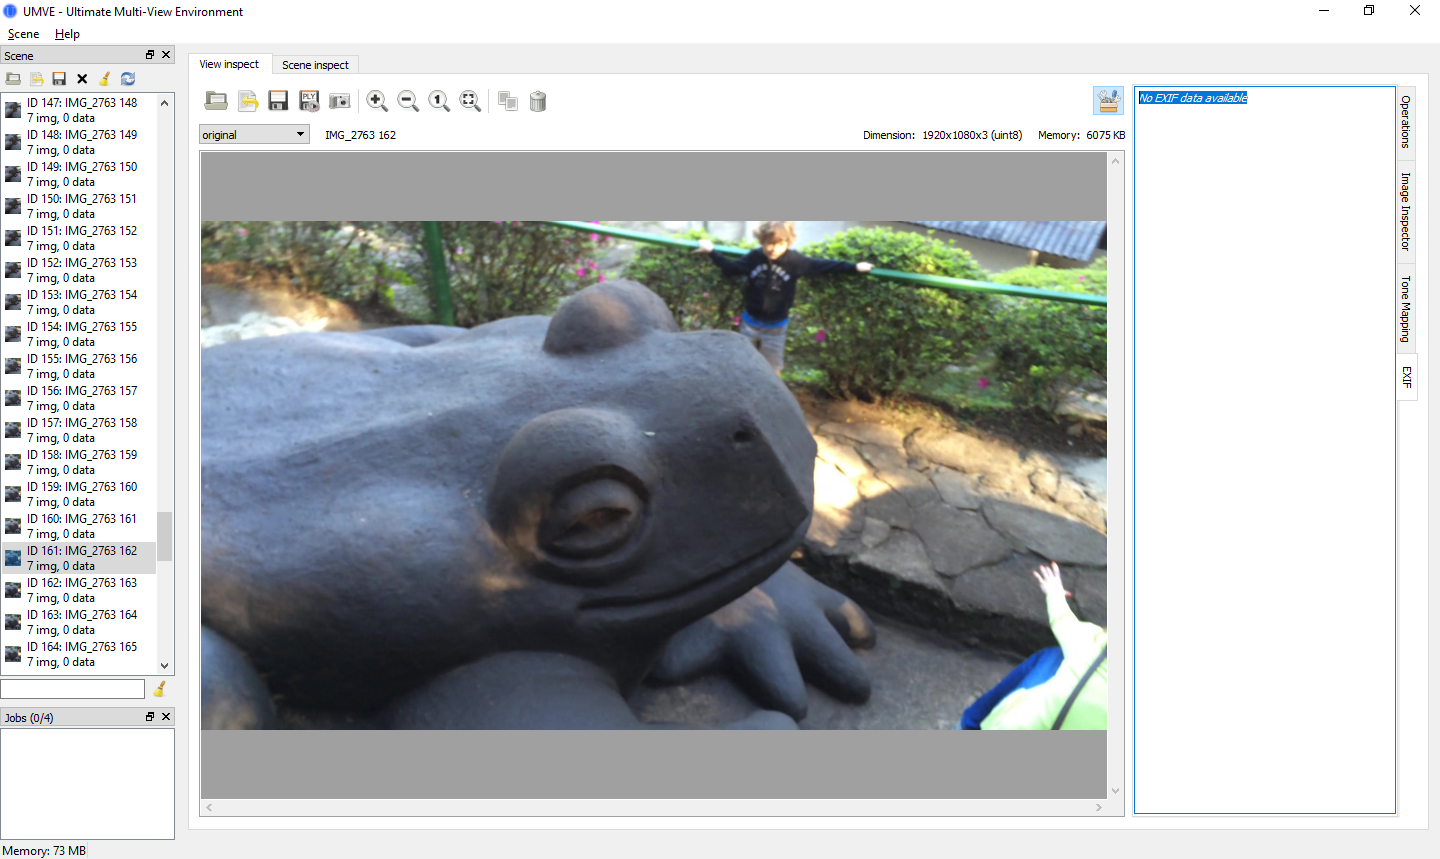
\includegraphics[width=0.461\linewidth]{figs/exifsemumve.png}(b)
	\caption{%
	A figura (a) é um exemplo onde a imagem possui dados na extensão \emph{EXIF} (destacado em azul). Ao passo que a figura (b) é um frame de um vídeo, que não possui os dados das câmeras (destacado em azul).
	%\cite{Cui:Theobalt:etal:PAMI2013,Pajdla:etal:ICCV2011}.
	}\label{fig:mveexif}
\end{figure} 

\newpage

Foi gerada uma reconstrução de um vídeo gravado de uma escultura no Jardim do Nêgo. O  vídeo foi cortado em \emph{frames} onde foram geradas 200 imagens base, com os parâmetros de câmera gerados pelo próprio software. 

A partir disso, foi executado, todos os passos de uma reconstrução utilizando o MVE, de forma que, foram utilizadas as duas opções, tanto por linha de comando, quanto pela interface gráfica (UMVE).

Pela interface gráfica, o processo todo de reconstrução foi rápido (cerca de 30 minutos) \ref{fig:UMVEdense}, ao passo que por linha de comando, levou cerca de 11 horas e 30 minutos, portanto, vamos nos atentar somente à reconstrução por linha de comando, onde, resumindo, tivemos os resultados~\ref{tab:mveSapo}. 

O UMVE não sinaliza quando o processo em execução termina, então, a explicação para essa discrepância no tempo é devido à execução de outro comando, sobrepondo o que já estava sendo executado, sem que o primeiro tivesse terminado.

\begin{figure}[!h]
	\centering
	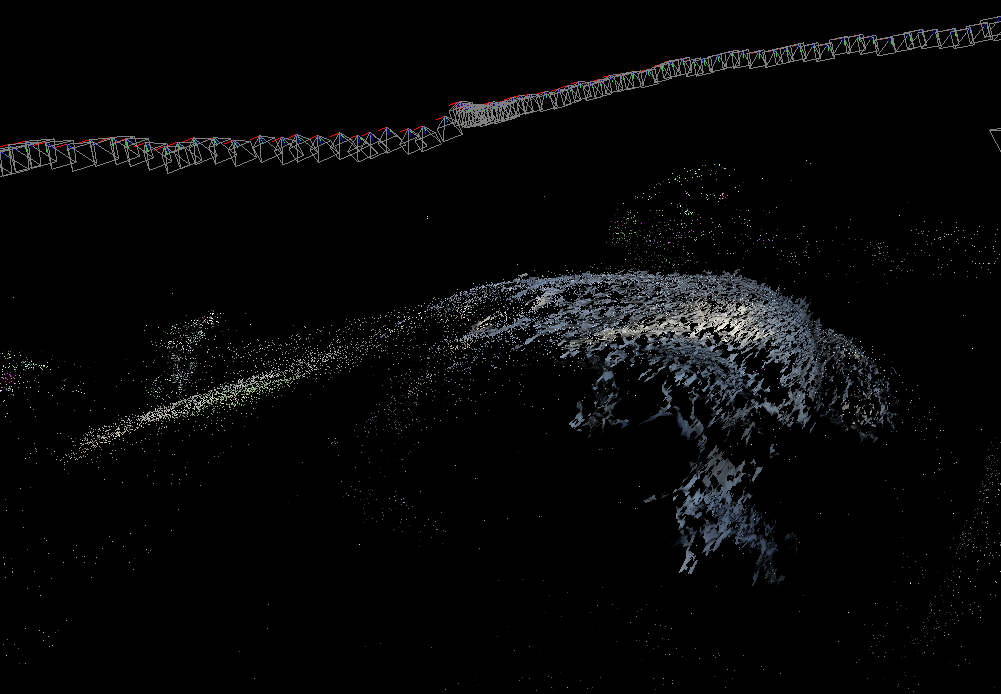
\includegraphics[width=\linewidth]{figs/umvedense.png}
	\caption{%
  Reconstrução final via UMVE; percebe-se que alguns pontos não foram
  considerados, mas o resultado geral foi uma nuvem de pontos mais densa.
  %\cite{Cui:Theobalt:etal:PAMI2013,Pajdla:etal:ICCV2011}.
	}\label{fig:UMVEdense}
\end{figure} 

\begin{table}[!h]
\centering
\caption{Tempos obtidos usando o MVE em um conjunto de dados do Jardim do Nêgo}
\label{tab:mveSapo}
\begin{tabular}{|l|l|}
\hline
Comando            & Tempo (aprox.)    \\ \hline
\emph{sfmrecon}  & 78 segundos     \\ \hline
\emph{dmrecon}   & 14.503 segundos \\ \hline
\emph{scene2pset} & 600 segundos    \\ \hline
\emph{fssrecon}  & 25.293 segundos \\ \hline
\emph{meshclean} & 60 segundos     \\ \hline
\end{tabular}
\end{table}

Na reconstrução por linha de comando também é possível visualizar em qual etapa da execução o algoritmo está (figura~\ref{fig:passosMVE}), configurar alguns parâmetros e inclusive mostrar a porcentagem de progresso do comando em execução. Foram executados os comandos declarados nesta seção.  O \emph{sfmrecon} demorou cerca de 1 minuto e meio \ref{fig:MVESfM}. 

\newpage

\begin{figure}[!h]
	\centering
	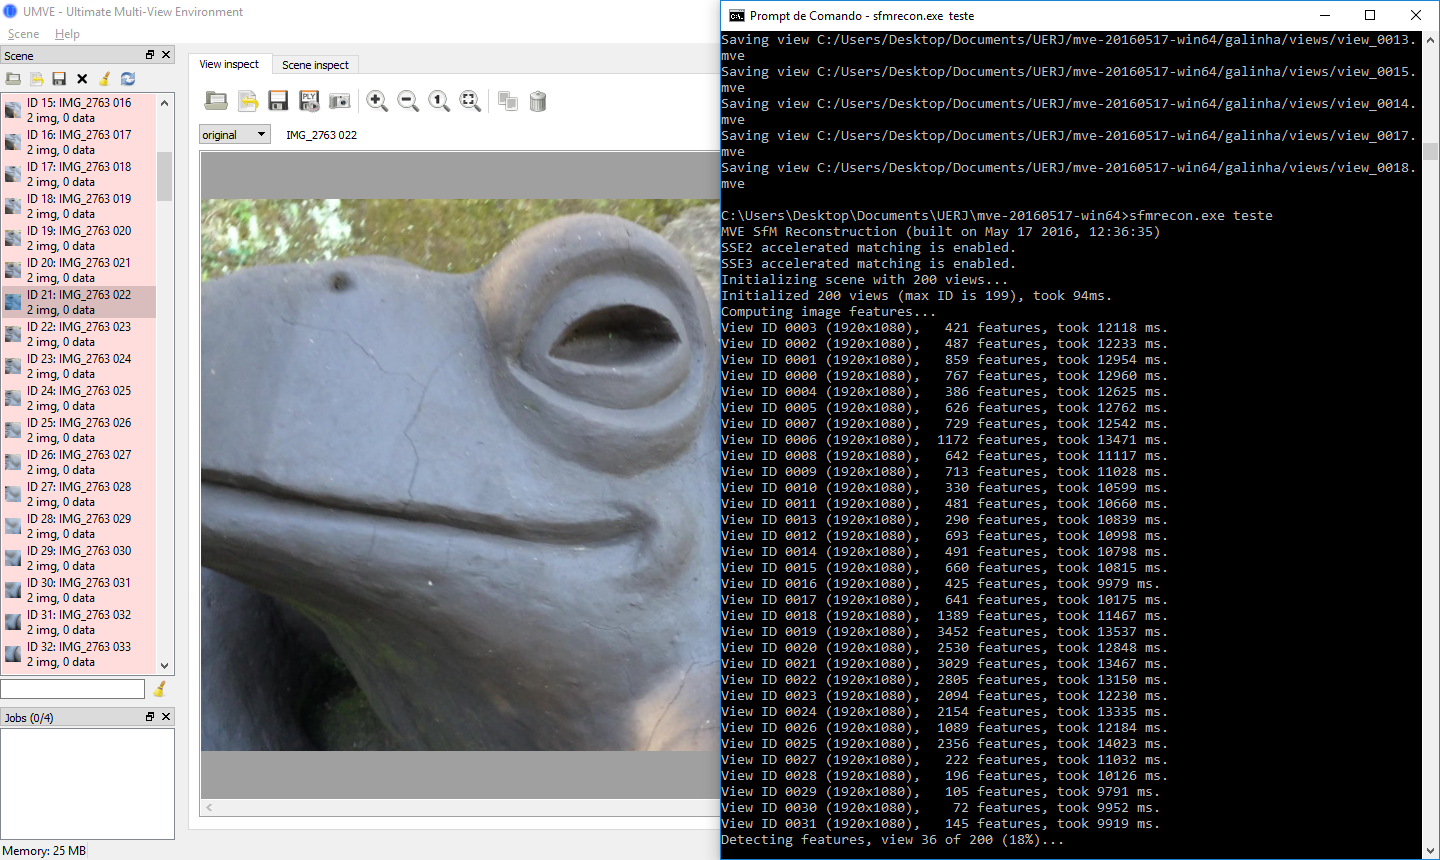
\includegraphics[width=0.45\linewidth]{figs/umve2sfm.png} (a)
	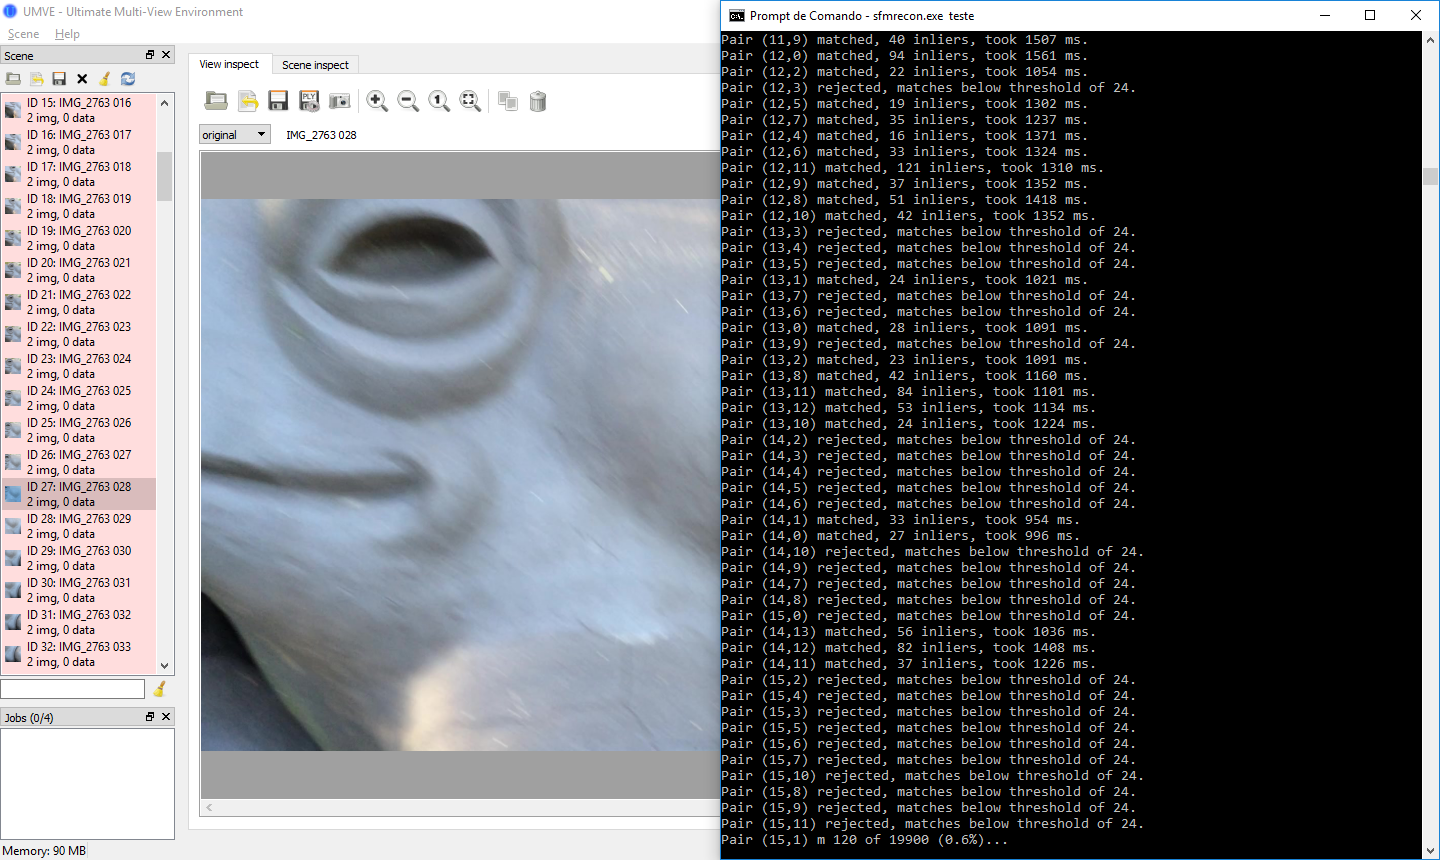
\includegraphics[width=0.45\linewidth]{figs/umve3sfmfeature.png} (b)
	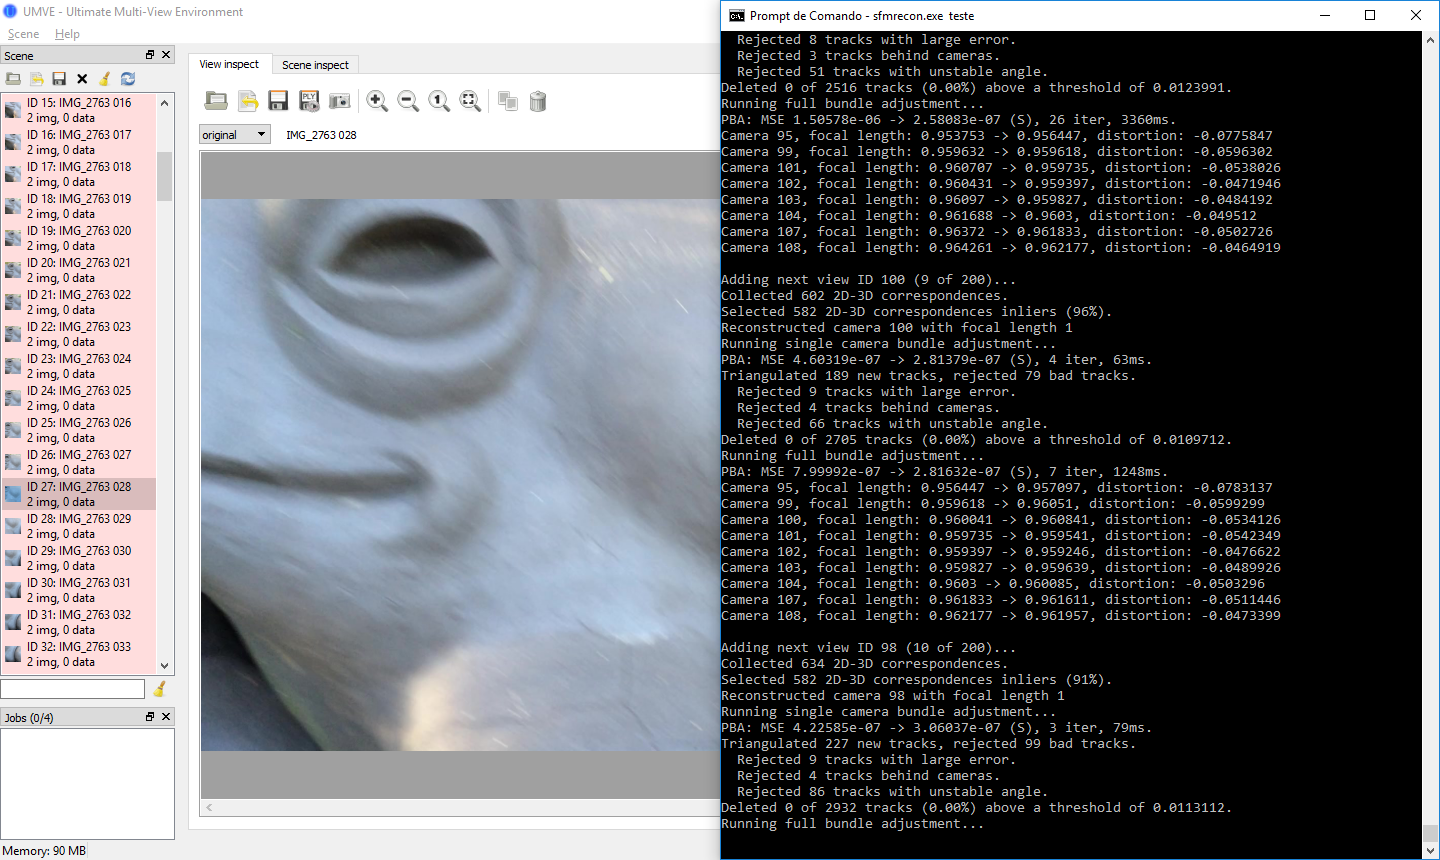
\includegraphics[width=0.45\linewidth]{figs/umve4ba.png} (c)
	\caption{%
	Processos dentro do comando \emph{sfmrecon}, onde (a) estão sendo detectadas as \emph{features} do conjunto de imagens. Em (b) está computado o \emph{pairwise matching} e em (c) está no processo de \emph{Bundle Adjustment}~\cite{bundleAdjustmentSlide}, usando condições-padrão para as câmeras.
	%\cite{Cui:Theobalt:etal:PAMI2013,Pajdla:etal:ICCV2011}.
	}\label{fig:passosMVE}
\end{figure} 

\begin{figure}[h!]
	\centering
	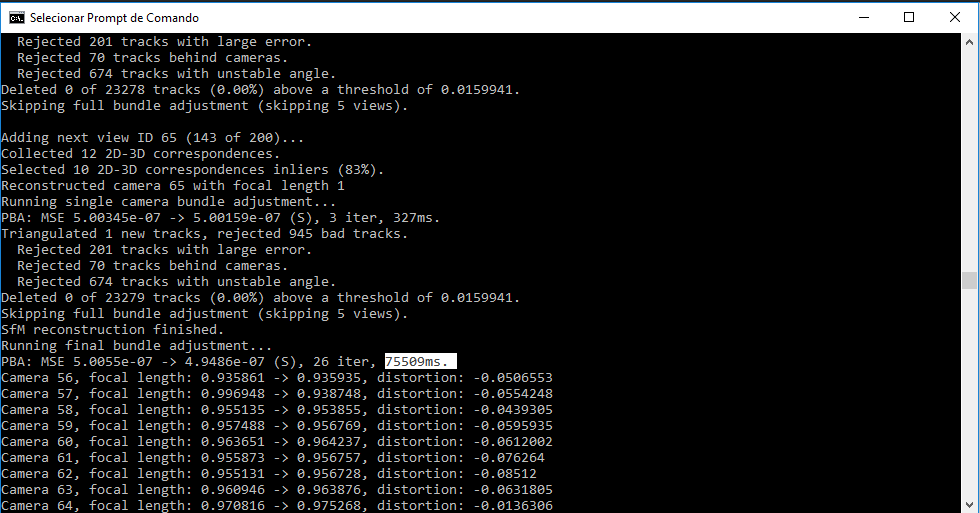
\includegraphics[width=0.65\linewidth]{figs/sfmmve.png}
	\caption{%
	Término do comando \emph{sfmrecon}, onde demorou cerca de 1 minuto e meio (75509 milisegundos).
	%\cite{Cui:Theobalt:etal:PAMI2013,Pajdla:etal:ICCV2011}.
	}\label{fig:MVESfM}
\end{figure}

O próximo comando, \emph{dmrecon} demorou cerca de 4 horas, usando como configuração um nível L2, com 20 vizinhos \ref{fig:MVEDenseRecon}. 
Usando um nível L0, o algoritmo rodou durante 6 horas aproximadamente e foi cancelado devido à demora na execução. 

\newpage

\begin{figure}[!h]
	\centering
	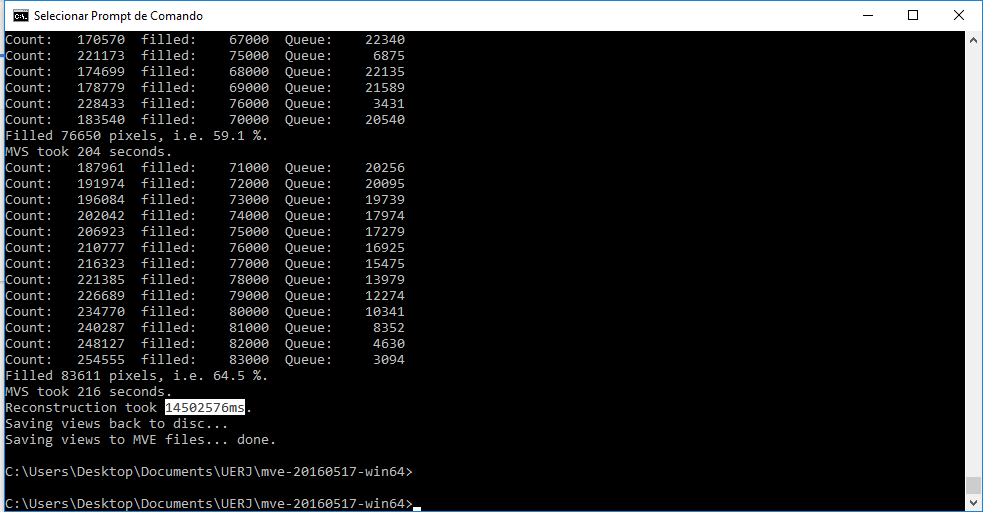
\includegraphics[width=0.8\linewidth]{figs/umvetempo.png}
	\caption{%
	Término do comando \emph{dmrecon}, onde demorou cerca de 4 horas (14502576 milisegundos).
	%\cite{Cui:Theobalt:etal:PAMI2013,Pajdla:etal:ICCV2011}.
	}\label{fig:MVEDenseRecon}
\end{figure} 

Usando o \emph{scene2pset}, é necessário especificarmos em qual nível estamos reconstruindo e também uma saída válida. Por exemplo: "scene2pset.exe -Fnivel cena output". Onde o nível poderá ser um 0 (-F0), 1 (-F1) e assim por diante, a cena é o \emph{input} e o \emph{output} é um arquivo de extensão configurável, neste caso \emph{.ply} \ref{fig:MVEscene2pset}. Este comando foi rápido, demorou cerca de 10 minutos, levando em conta todos os níveis.

\begin{figure}[!h]
	\centering
	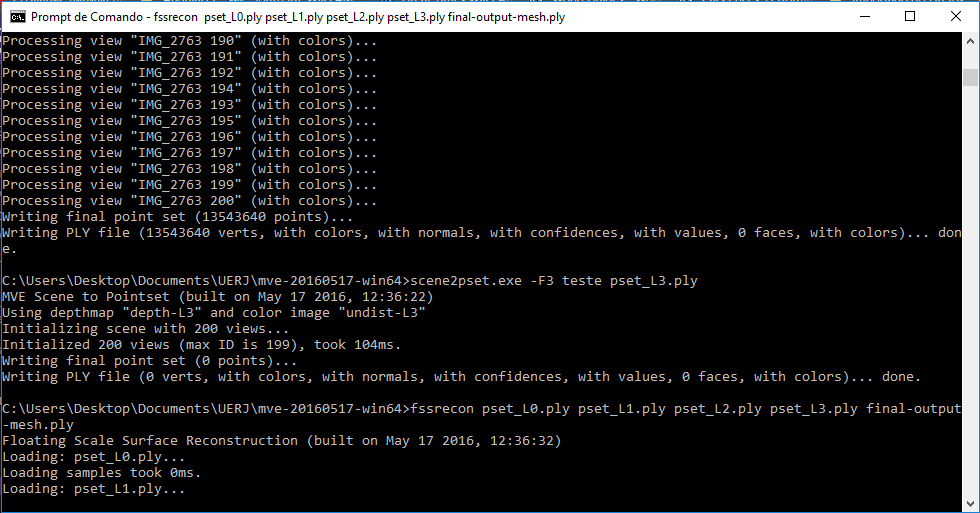
\includegraphics[width=0.8\linewidth]{figs/mvemesh.png}
	\caption{%
	Execução dos comandos \emph{scene2pset}, nos níveis -F0, -F1, -F2 e -F3.
	%\cite{Cui:Theobalt:etal:PAMI2013,Pajdla:etal:ICCV2011}.
	}\label{fig:MVEscene2pset}
\end{figure} 

Para juntar todos os níveis do \emph{scene2pset}, foi usado o \emph{fssrecon}, que gera uma única reconstrução. Este processo demorou bastante, cerca de 7 horas \ref{fig:MVEFSSR}. Que teve como resultado a malha \ref{fig:MVEFSSRMesh}.

\newpage

\begin{figure}[!h]
	\centering
	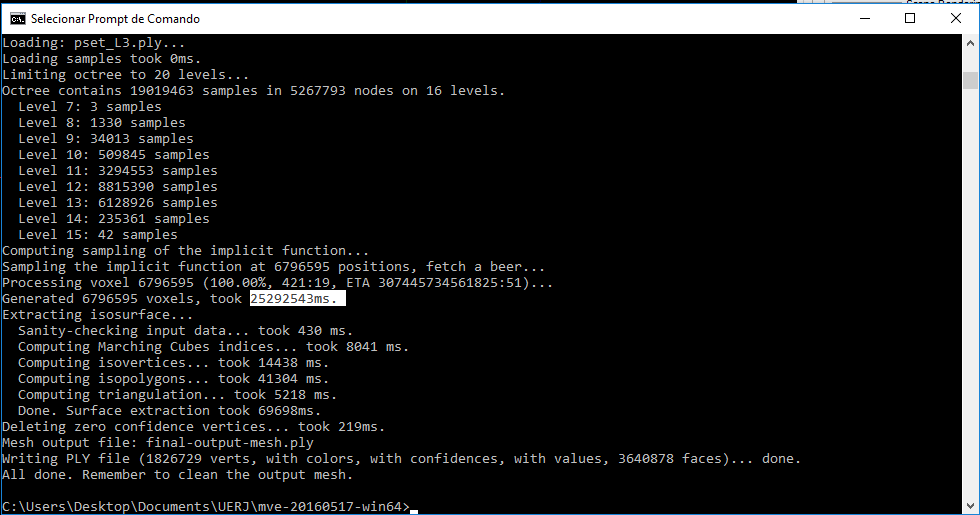
\includegraphics[width=0.8\linewidth]{figs/mvemeshtempo2.png}
	\caption{%
	Progressão do comando \emph{fssrecon}, onde possui o ETA -- \emph{Estimated Time of Arrival}.
	%\cite{Cui:Theobalt:etal:PAMI2013,Pajdla:etal:ICCV2011}.
	}\label{fig:MVEFSSR}
\end{figure} 

\begin{figure}[!h]
	\centering
	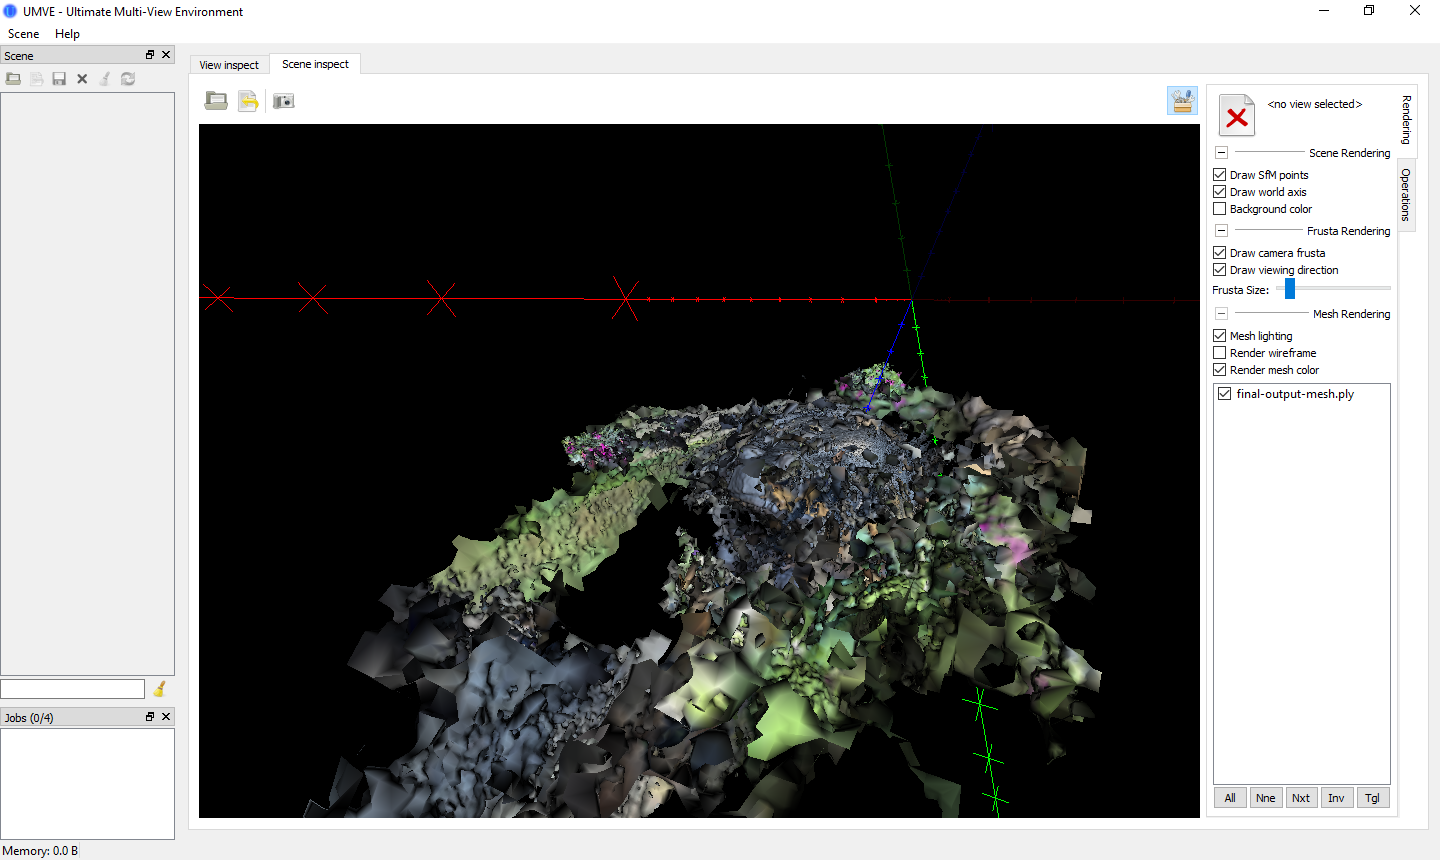
\includegraphics[width=1\linewidth]{figs/mvemeshout.png}
	\caption{%
	Malha com ruídos proveniente do comando \emph{fssrecon}.
	%\cite{Cui:Theobalt:etal:PAMI2013,Pajdla:etal:ICCV2011}.
	}\label{fig:MVEFSSRMesh}
\end{figure} 

Finalmente, basta limpar a malha atual com o comando \emph{meshclean}, onde foi obtido o resultado~\ref{fig:MVEMeshClean}.

\newpage

\begin{figure}[!h]
	\centering
	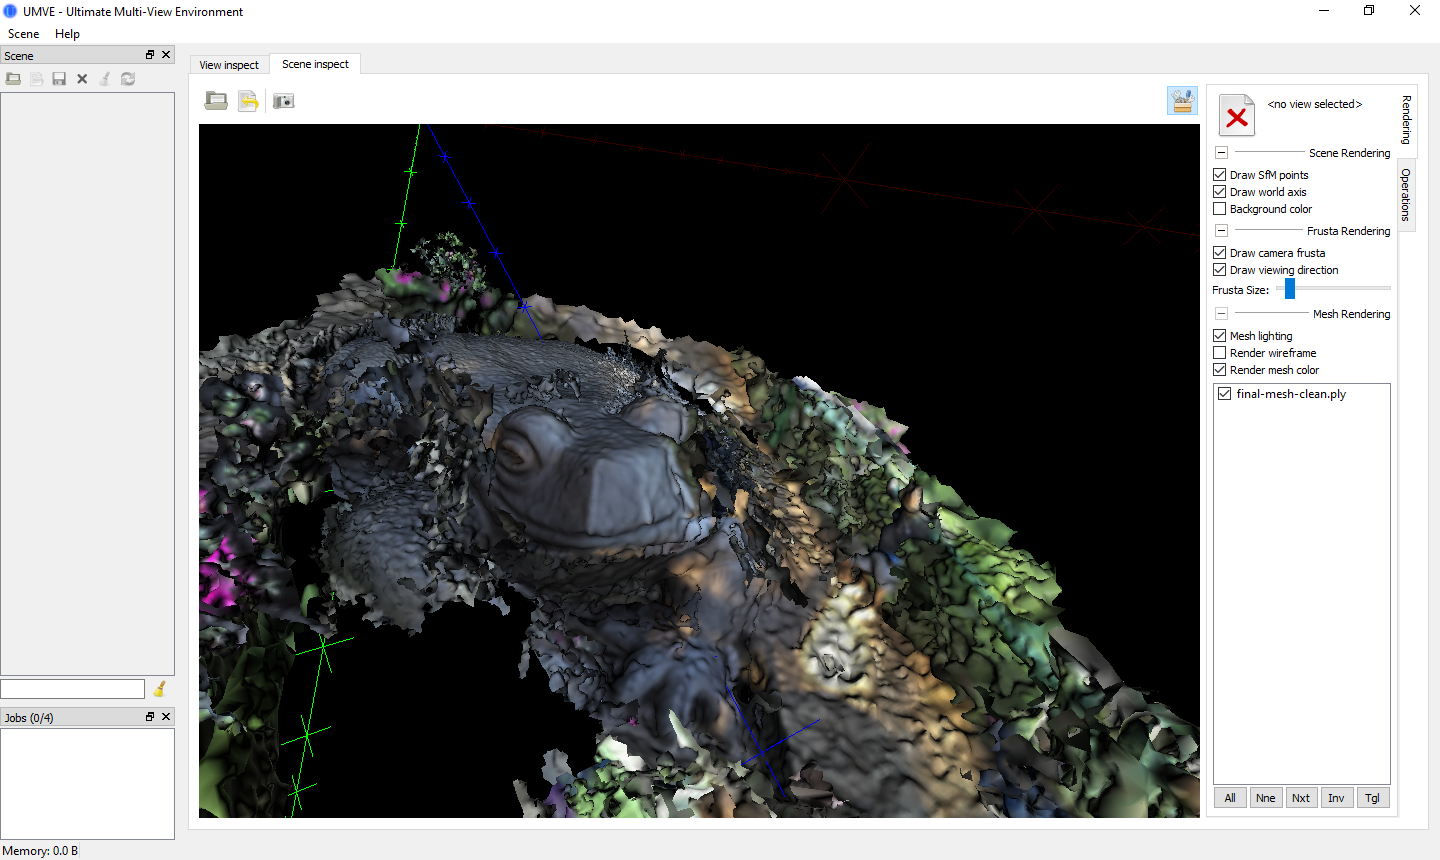
\includegraphics[width=1\linewidth]{figs/mvemeshclean.png}
	\caption{%
	Resultado final, após a remoção dos ruídos da malha.
	%\cite{Cui:Theobalt:etal:PAMI2013,Pajdla:etal:ICCV2011}.
	}\label{fig:MVEMeshClean}
\end{figure} 

Para comparação, usamos o mesmo objeto utilizado na reconstrução do VisualSfM (a galinha) e fizemos o passo a passo com o MVE: com a interface gráfica (UMVE), criamos uma nova cena e inserimos, primeiramente, as 200 fotos do objeto. Em seguida, utilizando as linhas de comando do MVE, fizemos o procedimento padrão de reconstrução do software. E, obtivemos os seguintes resultados~\ref{tab:galinha200mve}:

\begin{table}[!h]
\centering
\caption{Tempos obtidos usando o MVE em um conjunto de dados em ambiente interno com 200 imagens}
\label{tab:galinha200mve}
\begin{tabular}{|l|l|}
\hline
Comando            & Tempo (aprox.)         \\ \hline
\emph{sfmrecon}  & 371 segundos   \\ \hline
\emph{dmrecon}   & 3.716 segundos \\ \hline
\emph{scene2pset} & 300 segundos   \\ \hline
\emph{fssrecon}  & 1.695 segundos \\ \hline
\emph{meshclean} & 45 segundos    \\ \hline
\end{tabular}
\end{table}

\newpage

\begin{figure}[!h]
	\centering
	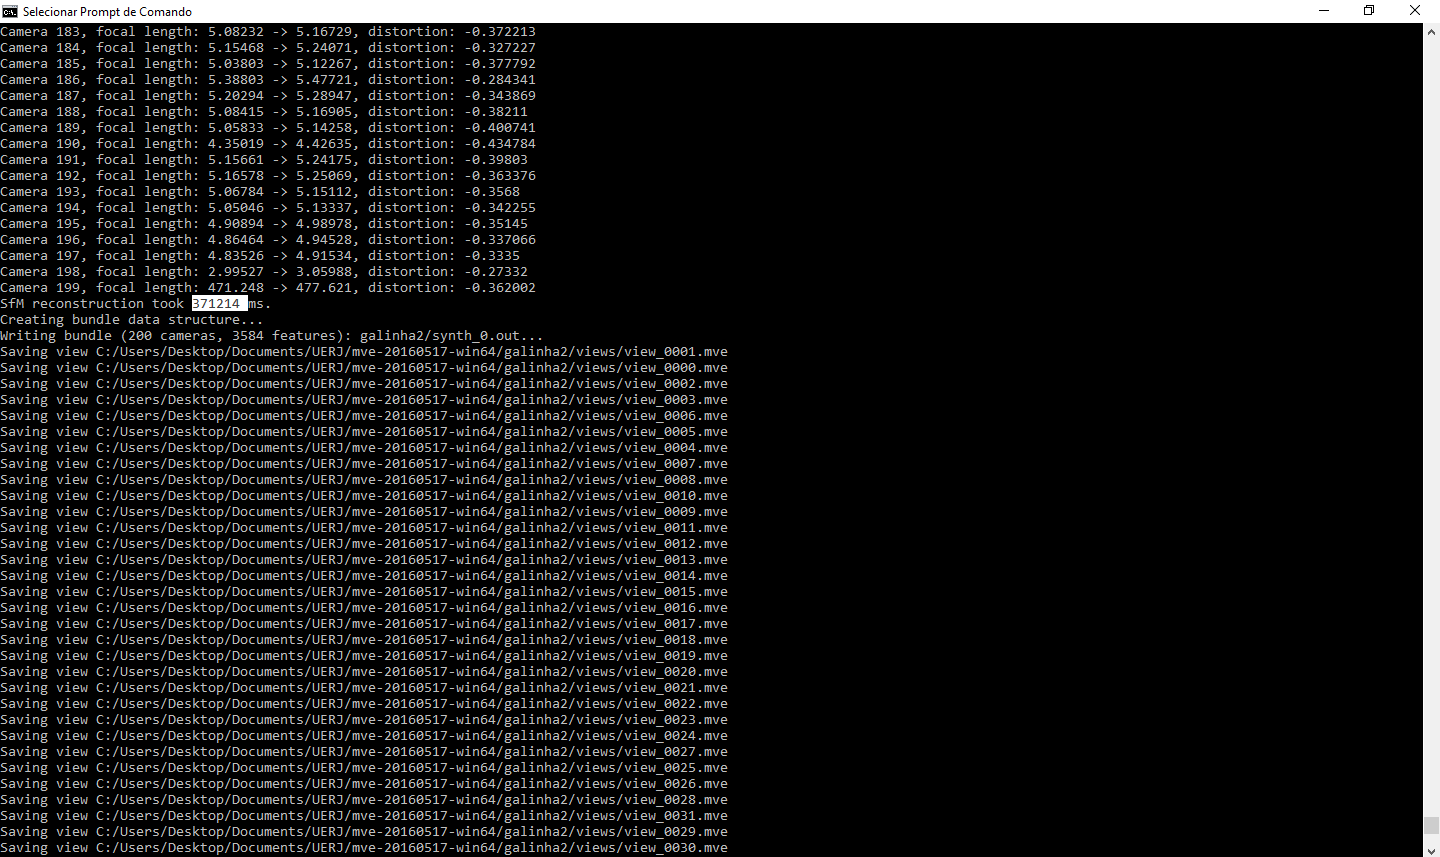
\includegraphics[width=0.5\linewidth]{figs/galinhalongesfmreconmve.png}
	\caption{%
	Tempo gasto da etapa \emph{sfmrecon} do MVE
	}\label{fig:sfmrecon1}
\end{figure}

\begin{figure}[!h]
	\centering
	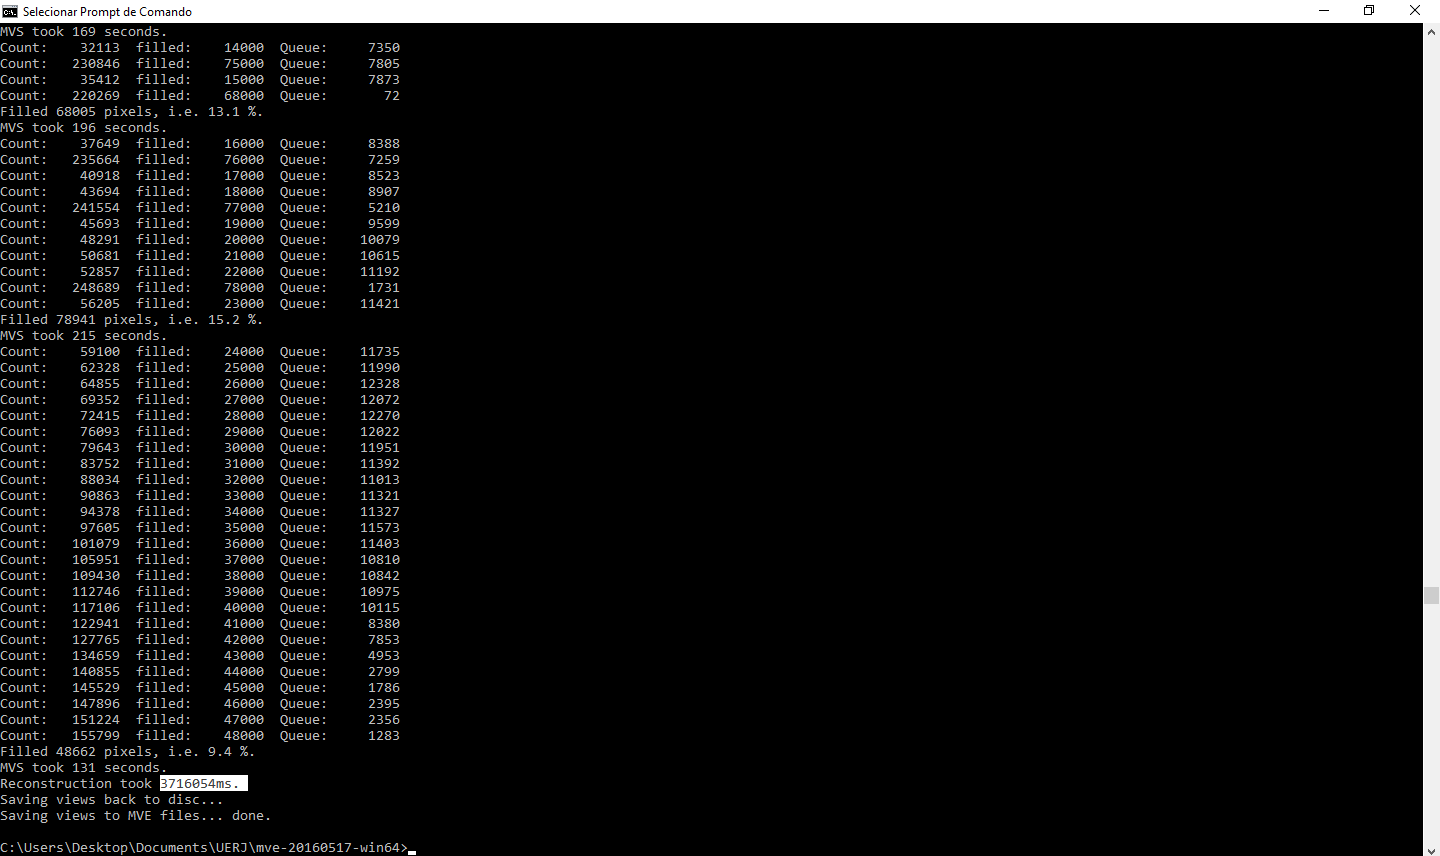
\includegraphics[width=0.5\linewidth]{figs/galinhadmreconmve.png}
	\caption{%
	Tempo da etapa \emph{dmrecon} do MVE
	%\cite{Cui:Theobalt:etal:PAMI2013,Pajdla:etal:ICCV2011}.
	}\label{fig:dmrecon1}
\end{figure}

\begin{figure}[!h]
	\centering
	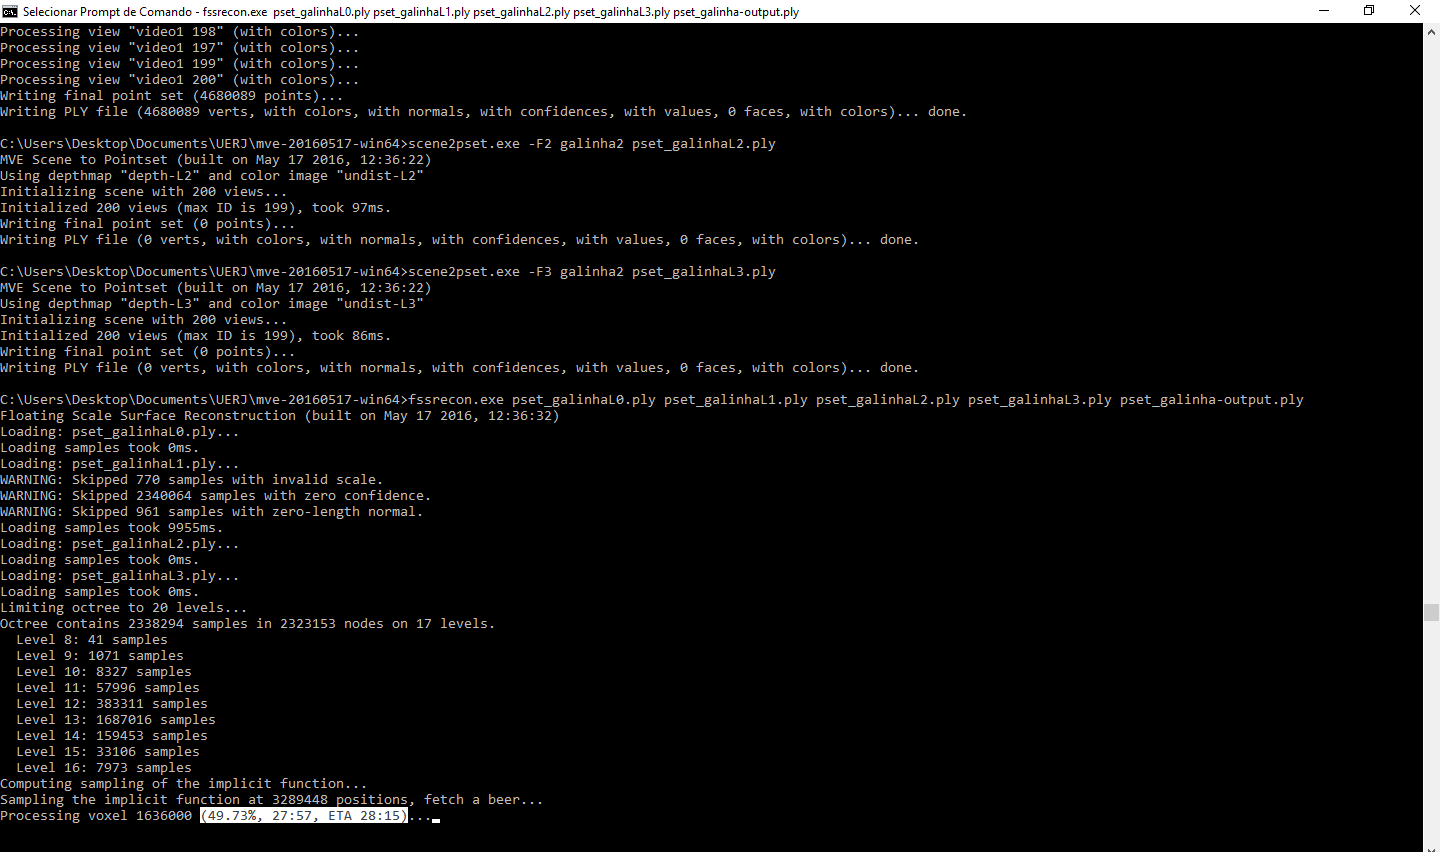
\includegraphics[width=0.7\linewidth]{figs/mvefssrecongalinha.png}
	\caption{%
	Tempo da etapa \emph{fssrecon} do MVE
	%\cite{Cui:Theobalt:etal:PAMI2013,Pajdla:etal:ICCV2011}.
	}\label{fig:fssrecon}
\end{figure}

\begin{figure}[!h]
	\centering
	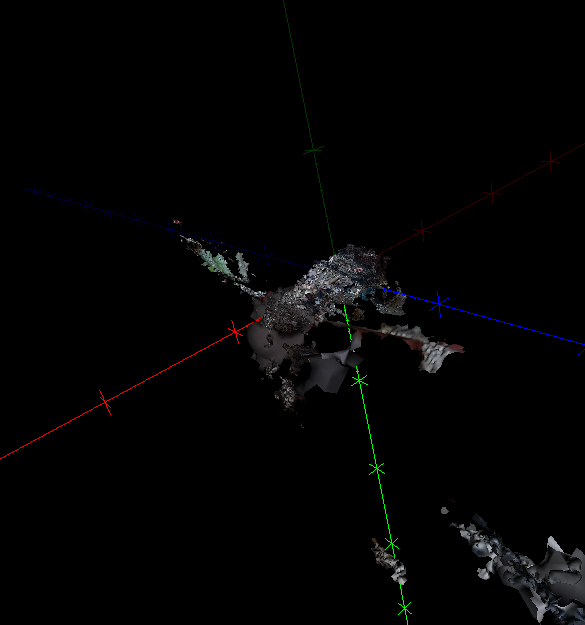
\includegraphics[width=0.7\linewidth]{figs/galinhadmr.png}
	\caption{%
	Resultado da etapa \emph{fssrecon} do MVE
	%\cite{Cui:Theobalt:etal:PAMI2013,Pajdla:etal:ICCV2011}.
	}\label{fig:galinhaFssr}
\end{figure}

\begin{figure}[!h]
	\centering
	\includegraphics[width=0.7\linewidth]{figs/galinhameshclean.png}
	\caption{%
	Resultado da etapa \emph{meshclean}, da etapa anterior \ref{fig:galinhaFssr}
	%\cite{Cui:Theobalt:etal:PAMI2013,Pajdla:etal:ICCV2011}.
	}\label{fig:galinhaMeshClean}
\end{figure}

\newpage

A etapa de \emph{scene2pset} demorou cerca de 20 segundos (total). Porém percebemos que a reconstrução não foi satisfatória, o \emph{software} se confundiu, e não conseguiu obter os parâmetros corretos das câmeras utilizadas. A partir disso, o erro se propagou e gerou essa reconstrução acima \ref{fig:galinhaFssr} e \ref{fig:galinhaMeshClean}.

Rodamos também, com as 224 fotos, só foi possível executar o passo \emph{sfmrecon} \ref{fig:galinhaSfM224}, pois o MVE não conseguiu rodar o comando \emph{dmrecon} por algum motivo, e não gerou nenhum resultado para a continuação do algoritmo \ref{fig:galinhaDMR224}.

\begin{figure}[!h]
	\centering
	\includegraphics[width=0.5\linewidth]{figs/mvesfmrecongalinhapertolonge.png}
	\caption{%
	Resultado da etapa \emph{sfmrecon}, com todas as imagens
	%\cite{Cui:Theobalt:etal:PAMI2013,Pajdla:etal:ICCV2011}.
	}\label{fig:galinhaSfM224}
\end{figure}

\begin{figure}[!h]
	\centering
	\includegraphics[width=0.5\linewidth]{figs/mvedmrecongalinhapertolonge.png}
	\caption{%
	Resultado da etapa \emph{dmrecon}, com todas as imagens
	%\cite{Cui:Theobalt:etal:PAMI2013,Pajdla:etal:ICCV2011}.
	}\label{fig:galinhaDMR224}
\end{figure}


%\chapter{Conclusão}
Técnicas práticas recentes de reconstrução 3D utilizando fotogrametria foram
apresentadas e exploradas, visando
ajudar a desenvolver os primórdios de um metodologia prática para digitalizar jardins de esculturas a céu
aberto. Foi adquirida experiência sobre a calibração de equipamentos, sistemas
de software recentes e esquemas para realizar uma boa varredura, cobrindo toda a
escultura com uma câmera comum de celular.  As esculturas Friburguenses visadas neste trabalho
possuem geometria peculiar, com curvas delineadas e regiões suaves, com pouca
textura e poucos pontos de interesse, sendo desafiadoras para o estado da arte
em escaneamento 3D; dessa forma, procuramos relatar as dificuldades e problemas
encontrados, para justificar a eventual pesquisa em novas técnicas mas
avançadas.

\section*{Trabalhos futuros} Identificamos os seguintes caminhos para a evolução deste projeto:
\begin{itemize}
\item \textbf{Realizar uma varredura com o Kinect.} Embora seja relativamente
  custoso, tanto fisicamente quanto computacionalmente, seria interessante ter
  um parâmetro de comparação prática das técnicas fotogramétricas passivas com
as técnicas de fotogrametria por Kinect, que se mostrou muito promissor em um
ambiente fechado.  
\item \textbf{Validação adicional.} Ter resultados mais
  expressivos, em questão quantitativa e não só qualitativa, para realizar uma
  engenharia mais completa do sistema, comparando valores em diferentes técnicas
  empregadas.
\item \textbf{Constatar na prática, a melhor estratégia de varredura de
  esculturas.}
Verificamos que um dos melhores modos de se escanear uma escultura de grande
porte seria escaneá-la várias vezes, de perto e de longe, a fim de que se pegue todos os detalhes,
cobrindo toda a área a ser reconstruída, e a fim de que a geometria global seja
bem restringida. Mas será que este é realmente o melhor método?  
\item \textbf{Realizar uma reconstrução de curvas.} 
  Utilizar uma reconstrução baseada em curvas para auxiliar na reconstrução de
  nuvem de pontos e superfícies densas, já que as esculturas do Jardim do Nêgo
  não possuem ampla informação pontual, mas sim de curvas e bordas. Nossos
  resultados indicam que aliar essas técnicas em um sistema de software ainda
  maior seria benéfico, além de constituir uma possível contribuição científica
  para publicação a curto prazo.
\item \textbf{Concretizar o objetivo proposto neste trabalho.} Ir mais vezes
  ao Jardim do Nêgo com o intuito de aumentar o acervo de filmes/imagens das
  esculturas de modo que seja possível ter uma reconstrução 3D satisfatória de
  todo o jardim, eternizando todo o patrimônio cultural.  
\item \textbf{Estratégia de larga escala.} De certa forma, os sistemas
  utilizados já são de
  larga escala (da ordem de centenas de imagens full HD), mas para escanear todo um jardim de esculturas em alta
  resolução, com uma metodologia prática facilmente replicável,
  será necessário empregar mais fortemente técnicas relacionadas a \emph{big data}, envolvendo o cluster do IPRJ
  e algoritmos de mais larga escala~\cite{Argarwal:Snavely:etal:ICCV09}. Pode-se pensar em um sistema em que o
  \emph{smartphone} faz upload dos vídeos na medida em que são capturados, os
  quais são reconstruídos incrementalmente usando o \emph{cluster} do IPRJ como nuvem computacional.
\end{itemize}
%======================================================================================
%Apresentamos um detector de borda subpíxel e um \textit{linker} de curvas projetado especificamente 
%para vídeos de água, aprendendo geometria e topologia em um conjunto de treinamento para 
%uso futuro como entrada para sistemas recentes de fotogrametria com base em curvas 3D.
%A abordagem modela o problema de forma que generaliza a criação de detectores
%específicos de \emph{features} geométricas para uma série de aplicações adicionais.
%As principais características do nosso sistema são: 1) Resolução ancorada nas
%singularidades para reconstruções nítidas; e 2) Treinamento de distribuições de
%geometria de contorno que permitem melhorias no rastreamento da água.
%
%\section*{Trabalhos futuros} Identificamos os seguintes caminhos para evolução deste trabalho:
%\begin{itemize}
%  \item \textbf{Realizar a aprendizagem em 3D.} Isso envolveria a marcação manual 
%    das bordas confiáveis em 3D, em cima de uma reconstrução de desenho 
%    3D~\cite{Usumezbas:Fabbri:Kimia:CVPR17,Usumezbas:Fabbri:Kimia:ECCV16}, ou 
%    marcando correspondências nas imagens. Nosso grupo de pesquisa já possui 
%    uma GUI para isso, mas a aprendizagem deve ser adaptada. As vantagens de 
%    fazer a aprendizagem em 3D é que o computador não precisa aprender 
%    invariantes projetivos e pode se concentrar diretamente na geometria verdadeira.
%  \item \textbf{Validação adicional.} Seria desejável produzir uma pontuação de erro 
%    no treinamento e examinar os valores atípicos de forma mais próxima, a fim de 
%    realizar uma engenharia mais completa do sistema.
%  \item \textbf{Aplicação em imagens ao ar livre.} Nosso conjunto de dados e 
%    configuração de aquisição de vídeo foi construído para imagens internas, mas 
%    gostaríamos de ter um sistema de aquisição ao ar livre. Existem dois cenários:
%    \begin{itemize}
%      \item Usuário final em uma praia: tenha quatro smartphones no modo de vídeo dispostos 
%        verticalmente em um pólo, auto-calibrados e sincronizados por um clique de som.
%      \item Plataforma de óleo: várias câmeras auto-calibradas monitorando condições do mar.
%    \end{itemize}
%  \item \textbf{Escala da arquitetura do sistema.} Seria importante paralelizar o processamento 
%    dos vídeos além da abordagem quadro a quadro e orientada a E/S descrita
%    neste trabalho.
%  \item Automatizar o recorte da região de interesse do vídeo.
%  \item Tornar os parâmetros de comprimento relativos ao tamanho da imagem.
%\end{itemize}

% ----------------------------------------------------------
% ELEMENTOS POS-TEXTUAIS
% ----------------------------------------------------------



% ----------------------------------------------------------
% ELEMENTOS POS-TEXTUAIS
% ----------------------------------------------------------

\backmatter

% ----------------------------------------------------------
% Referencias
% ----------------------------------------------------------

%\citeoption{bibliografia}
\bibliography{rf-multiview,personal,Kimia,indexing,vision,categorization,edge,recognition,segmentation,edge-linking,proceedings}

% ----------------------------------------------------------
% Glossario
% ----------------------------------------------------------

%\glossario
%======================================================================================
%\postextualchapter*{Glossário}
%======================================================================================

%\definicao{bit}{A menor unidade de informação computacional, podendo assumir os valores 0 ou 1}

% ----------------------------------------------------------
% Apendices
% ----------------------------------------------------------

% ---
% Inicia os apêndices
% ---
\appendix

%======================================================================================
%\postextualchapter{Primeiro apêndice}
%======================================================================================


% ----------------------------------------------------------
% Anexos
% ----------------------------------------------------------

% ---
% Inicia os anexos
% ---
\annex

%======================================================================================
\postextualchapter{Vídeos dos tanques de ondas}
%======================================================================================
(Os quatro vídeos dos tanques de ondas encontram-se junto deste material gravados em DVD.)

%---------------------------------------------------------------------
% INDICE REMISSIVO
%---------------------------------------------------------------------

\printindex

\end{document}
